% !TEX program = xelatex
\documentclass[12pt,a4paper]{ctexart}

% ── Packages ──
\usepackage[top=2.5cm,bottom=2.5cm,left=2.8cm,right=2.8cm]{geometry}
\usepackage{graphicx}
\usepackage{booktabs}
\usepackage{array}
\usepackage{hyperref}
\usepackage{amsmath,amssymb}
\usepackage{multirow}
\usepackage{caption}
\usepackage{subcaption}
\usepackage{enumitem}
\usepackage{xcolor}
\usepackage{longtable}

\hypersetup{
    colorlinks=true,
    linkcolor=blue,
    citecolor=blue,
    urlcolor=blue,
}

\graphicspath{{figures/}}

% ── Title ──
\title{\bfseries 基于深度学习的A股股票排序预测与模拟交易\\
        ——双路线探索与对比分析}
\author{
    PB24050961\;李沐泽$^{1}$ \quad
    PB24030836\;吴鸿哲$^{2}$ \quad
    PB24261889\;王俊涛$^{3}$
}
\date{\today}

\begin{document}

\maketitle
\n\tableofcontents
\newpage

\begin{abstract}
\noindent
本文记录了深度学习课程大作业中，对A股股票横截面收益预测任务的系统性探索。
项目采用两条独立的技术路线：路线A以GRU为骨干网络，配合稀疏空间注意力（Sparse Spatial Attention）
和ListMLE排序损失，经过V1至V9共九个版本的迭代优化；路线B以CNN-LSTM为骨干网络，
聚焦于归一化方案对比与训练数据规模对泛化能力的影响。
两条路线在统一的回测框架下进行了定量对比。
本文重点阐述各版本的设计动机、技术决策依据、失败尝试的根因分析，以及两条路线在方法论层面的互补性。
最终模型在验证集上取得了Rank IC 0.106的排序质量，
路线A在含成本的历史回测中实现累计净收益+23.7\%（N=10, 94个交易日）。
\end{abstract}

% ═══════════════════════════════════════════════════════════
\section{项目背景与问题定义}
% ═══════════════════════════════════════════════════════════

\subsection{任务背景}

金融时间序列具有高噪声、非平稳性和复杂依赖结构，是深度学习实际应用中的典型挑战场景。
A股市场作为全球第二大股票市场，截至2026年拥有约5,000只上市股票，
其特有的T+1交易机制、涨跌停限制以及散户主导的交易结构，使得预测建模面临独特困难。

本项目以A股全市场股票为研究对象，利用深度学习模型在每日收盘后对全市场股票进行横截面排序预测，
基于预测得分驱动T+1轮动交易策略，并在2026年6月1日至12日的模拟交易比赛中进行实战验证。

\subsection{任务定义}

给定股票$i$在交易日$t$过去$T$个交易日的特征序列
$\mathbf{X}_{i,t} \in \mathbb{R}^{T \times D}$，
预测其在$t+1$日的横截面排序得分$s_{i,t+1}$。

模型输出的排序得分直接用于N-K轮动策略：
每日卖出当前持仓中得分最低的$K$只股票，
买入全市场得分最高的$K$只股票，维持$N$只等权持仓。
这种策略的核心假设是：模型预测的排序质量是策略收益的主要驱动力，
精确的价格预测并非必要——能够可靠地判断“A比B更可能上涨”即可驱动交易。

\subsection{数据来源与股票池过滤}

数据来源于课程提供的A股全市场日频数据，覆盖2016年1月至2026年6月，约5,517只股票。
基础数据字段包括：开盘价、最高价、最低价、收盘价（OHLC）以及成交量和成交额。
进阶数据包括基本面指标（市盈率PE、市净率PB、流通市值等）和资金流向数据。

进入模型训练前，两条路线执行共同的前置过滤流程：
\begin{itemize}[leftmargin=*]
    \item \textbf{剔除ST、*ST及退市股}：263只，通过股票名称关键词匹配过滤
    \item \textbf{剔除北交所股票}：313只，北交所流动性较低、交易规则差异较大
    \item \textbf{剔除长期停牌股}：单只股票内最大日期间隔超过365天的股票被剔除（如\verb|000029.SZ|曾停牌1,518天）
    \item \textbf{剔除短历史新股}：总数据行数少于120行的次新股被剔除，确保滑动窗口构造有足够数据
\end{itemize}

最终股票池约4,940只，覆盖2016年起持续交易的老股以及逐年上市的新股。
其中52.5\%的股票（2,597只）完整覆盖了整个数据期。

\subsection{预测标签构造}

路线A采用T+1日收益率作为预测目标：
\begin{equation}
    y_{i,t} = \frac{\text{close}_{i,t+1} - \text{close}_{i,t}}{\text{close}_{i,t}}
\end{equation}
其中$\text{close}_{i,t}$为股票$i$在第$t$日的收盘价（复权后）。
选择T+1标签的核心原因在于诚实性：早期版本曾使用T+5累计收益率作为标签，
虽然验证集IC更高（0.113 vs 0.106），但该优势源于训练期（2019--2024）的动量溢价而非真实预测能力，
2026年动量断裂后T+5的测试IC暴跌至0.010。

路线B采用T+1收盘价作为预测目标，通过
$\hat{r}_{t+1} = \hat{p}_{t+1} / p_t - 1$反算预期收益率进行排序。

\subsection{数据集划分}

两条路线均采用严格的时间序列划分，杜绝任何形式的未来信息泄漏：

\begin{itemize}[leftmargin=*]
    \item \textbf{路线A}：训练集2019--2024（6年），验证集2025全年，测试期2026年1月5日至5月29日（94个交易日）
    \item \textbf{路线B}：采用2024--2026三年混合训练（约192万样本），
          每只股票前80\%为训练、训练末10\%为验证、后20\%为测试，
          按股票级别划分，确保同一只股票的窗口不会跨训练/测试集
\end{itemize}

关键约束：训练集和验证集之间严格按时间切分，禁止随机打乱。
样本构造采用滑动窗口方式，数据标准化在窗口级别进行，不使用全量数据计算均值和方差。

\subsection{数据泄露防护}

两条路线均在各环节进行了数据泄露的防护设计，汇总如表\ref{tab:leak_prevention}。

\begin{table}[htbp]
\centering
\caption{数据泄露防护措施汇总}
\label{tab:leak_prevention}
\begin{tabular}{lp{5cm}p{5cm}}
\toprule
防护环节 & 路线A & 路线B \\
\midrule
归一化 & 两阶段归一化：时序特征per-window Z-score，截面特征per-date Z-score（V5修复了截面特征的归一化缺陷） & 因果Max-Min归一化：每只股票独立，只用截至当日的历史极值计算缩放 \\
数据集划分 & 按时间切分（2019--2024训练，2025验证），禁止随机打乱 & 按股票级别切分（前80\%训练，后20\%测试），不跨股票混合 \\
滑动窗口 & 窗口内标准化，不使用全量统计量 & 窗口内标准化，不使用全量统计量 \\
标签构造 & T+1收益率基于次日收盘价，不使用未来价格 & 因果累积极值（非全局），不含未来信息 \\
\bottomrule
\end{tabular}
\end{table}

\subsection{交易成本模型}

路线A在回测中采用净值成本模型，费用构成如表\ref{tab:cost_model}所示。

\begin{table}[htbp]
\centering
\caption{交易成本明细}
\label{tab:cost_model}
\begin{tabular}{lcc}
\toprule
费用项 & 卖出（/支） & 买入（/支） \\
\midrule
印花税 & 0.05\% & — \\
佣金（万2.5） & 0.025\% & 0.025\% \\
过户费 & 0.001\% & 0.001\% \\
\midrule
单边合计 & 0.076\% & 0.026\% \\
\bottomrule
\end{tabular}
\end{table}

成本按净变化计算：同只股票的买卖不重复计费，净变化部分分摊至$N$只持仓。
路线B的回测在统一框架下采用相同成本模型（详见第五章）。

\subsection{评测指标体系}

评测分为四个层级：

\textbf{Tier 1 — 信号质量（不依赖策略参数）：}
\begin{itemize}[leftmargin=*]
    \item \textbf{Rank IC}：模型预测分数与次日收益率的Spearman秩相关系数，每日计算后取均值
    \item \textbf{ICIR}：IC均值除以IC标准差，衡量信号稳定性
    \item \textbf{IC > 0 比例}：IC为正的交易日占比
    \item \textbf{月度IC分解}：按月份拆分的IC均值，观察信号时间衰减
\end{itemize}

\textbf{Tier 2 — 策略表现：}
\begin{itemize}[leftmargin=*]
    \item \textbf{累计收益率}：期初100万资金，期末终值
    \item \textbf{年化收益率}：按252个交易日年化
    \item \textbf{夏普比率（Sharpe Ratio）}：年化超额收益与年化波动率之比
    \item \textbf{最大回撤（Max Drawdown）}：累计收益从峰值到谷底的最大跌幅
\end{itemize}

\textbf{Tier 3 — 风险与稳定性：}
\begin{itemize}[leftmargin=*]
    \item \textbf{月度收益分解}：按月份拆分的净收益
    \item \textbf{日胜率}：日收益为正的交易日占比
    \item \textbf{滚动窗口表现}：10日滚动窗口的胜率与最差窗口
\end{itemize}

\textbf{Tier 4 — 成本效率：}
\begin{itemize}[leftmargin=*]
    \item \textbf{Gross→Net损耗}：交易成本对总收益的侵蚀
    \item \textbf{日均换手率}：每日调仓股票占持仓的比例
\end{itemize}

% ═══════════════════════════════════════════════════════════
\section{数据预处理与特征工程}
% ═══════════════════════════════════════════════════════════

两条路线在共同的前置过滤（第一章已详述）基础上，选择了截然不同的特征工程策略。
路线A追求特征的丰富性和可解释性，路线B追求特征的简约性和端到端学习能力。

\subsection{路线A：26维多源特征融合}

路线A构建了包含量价、技术指标、截面排名和估值指标的四类特征体系，
总计26维输入特征（19维时序 + 7维截面），如表\ref{tab:routeA_features}所示。

\begin{table}[htbp]
\centering
\caption{路线A特征体系（26维）}
\label{tab:routeA_features}
\small
\begin{tabular}{lll}
\toprule
类别 & 特征 & 维度 \\
\midrule
量价（时序） & open, high, low, close, vol, amount, pct\_chg, & 10 \\
             & turnover\_rate, volume\_ratio, total\_mv & \\
技术指标（时序） & MACD, MACD\_signal, RSI, BB\_width, BB\_pct, & 8 \\
                & MOM\_5, MOM\_20, VOL\_20 & \\
vwap\_gap（时序） & close/vwap - 1（机构活动代理信号） & 1 \\
\hline
截面排名 & rank\_pct(pct\_chg), rank\_pct(amount), & 4 \\
          & rank\_pct(turnover\_rate), pct\_chg - CSI300\_ret & \\
估值截面 & rank\_pct(PE), rank\_pct(PB), rank\_pct(circ\_mv) & 3 \\
\midrule
合计 & & \textbf{26} \\
\bottomrule
\end{tabular}
\end{table}

\subsubsection{两阶段归一化}

路线A的归一化体系是经历V5版本重构后确立的核心设计，解决了此前截面特征因归一化顺序错误
而全部退化为零向量的关键缺陷。

\begin{itemize}[leftmargin=*]
    \item \textbf{时序特征（per-window Z-score）}：每个滑动窗口内沿时间轴（$T$轴）独立计算均值和标准差进行Z-score归一化。
          这确保了不同股票的时间序列模式在同一尺度上可比，且不依赖未来窗口数据。
    \item \textbf{截面特征（per-date Z-score）}：每个交易日内沿股票横截面（$N$轴）独立计算均值和标准差进行Z-score归一化后，
          再复制（tile）到时间维度。截面排名值（如PE排位）在单一交易日内的所有股票间具有可比性，
          应先在截面上归一化，再扩展到时间轴。此前V1--V4将这个顺序颠倒——
          先将截面值tile到60个时间步，再经受per-window Z-score，导致每个时间步上所有股票共享同一常数，
          标准差为零，归一化后全部退化为零。
    \item \textbf{估值PE/PB做clip截断}：PE限制在[0.1, 500]，PB限制在[0.1, 50]，防止极端值扭曲排名。
\end{itemize}

\subsubsection{预处理增强}

除归一化外，路线A还进行了如下预处理增强：

\begin{itemize}[leftmargin=*]
    \item \textbf{log1p变换}：对成交量（vol）、成交额（amount）和总市值（total\_mv）做$\log(1+x)$变换，
          将长尾分布压缩到更接近正态分布的范围
    \item \textbf{Winsorization}：对时序特征做1\%/99\%分位截断，抑制异常日（如涨跌停）的极端值对特征分布的扭曲
    \item \textbf{缺失值处理}：原始量价列做前向填充（ffill），缺PE/PB的股票截面排名默认返回0.5（中性排位），
          避免NaN在特征张量中传播
\end{itemize}

\subsection{路线B：1维极简特征}

与路线A的多维融合策略形成鲜明对比，路线B选择了极致的特征简约：
仅使用归一化后的收盘价序列（1维）作为CNN-LSTM模型的输入。

\subsubsection{因果累积Max-Min归一化}

路线B的核心创新是一种严格因果的归一化方法，对每只股票独立计算渐进的Min-Max缩放：

\begin{equation}
\text{scaled}[i] = \frac{\text{close}[i] - \min_{j \le i}(\text{close}[j])}
                         {\max_{j \le i}(\text{close}[j]) - \min_{j \le i}(\text{close}[j])}
\end{equation}

该方法的关键特性：
\begin{itemize}[leftmargin=*]
    \item \textbf{按股票独立}：每只股票各自维护min/max累积值，天然消除不同股票间的绝对价格差异（如1元股与100元股不可直接比较的难题）
    \item \textbf{因果约束}：仅使用截至当前日的历史极值，保证无未来信息泄漏——缩放参数为$\text{min\_ref}$和$\text{max\_ref}$的滚动窗口值
    \item \textbf{噪声注入}：训练集（前80\%）在缩放值上施加乘性高斯噪声$\mathcal{N}(0, 0.03)$，增强模型对缩放参数微小偏移的鲁棒性
    \item \textbf{输出区间}：$[0, 1]$闭区间
\end{itemize}

归一化后，采用序列长度$T=20$的滑动窗口将收盘价序列构造为模型输入样本。

\subsubsection{Sigmoid全局归一化的系统性失效}

路线B在归一化方案的探索中，系统性地对比了另一种方案——全局Sigmoid归一化——并发现其在A股市场完全无效，
这一对比本身构成了重要的方法论贡献。

Sigmoid方案使用全局参数$\text{start}=0$和$\text{end}=500$将全市场股票价格映射到$(0,1)$区间，
变换公式为：
\begin{equation}
\text{score} = \frac{2}{1 + \exp\left(-\ln(40000) \cdot \frac{x-500}{500} + \ln(0.005)\right)} \cdot \frac{1}{2}
\end{equation}

该方案的失效源于三个不可调和的设计缺陷：

\begin{enumerate}[leftmargin=*]
    \item \textbf{分布错位}：A股市场93.38\%的股票收盘价$\le$52元，全部落在Sigmoid左侧平缓区，
          不同股票间的缩放值几乎不可区分，模型的输入丧失了股票间的区分度。
    \item \textbf{全局参数不灵活}：单一$\text{end}=500$的参数无法同时适配1元低价股和100元以上高价股。
          若放宽$\text{end}$以容纳高价股，则低价股区间被过度压缩。
    \item \textbf{极端值拖垮分辨率}：全市场最高价达2,601元，迫使$\text{end}$取一个远大于主流股价范围的值，
          导致绝大部分股票的缩放值被挤在一个极窄区间内。
\end{enumerate}

实验验证了该结论（表\ref{tab:sigmoid_vs_maxmin}）：在同一CNN-LSTM模型和3年混合训练配置下，
Max-Min因果归一化的IC达到0.118（Rank IC 0.088），方向胜率52.5\%；
而Sigmoid归一化的IC仅为-0.016（Rank IC -0.008），方向胜率48.9\%——接近随机水平。

\begin{table}[htbp]
\centering
\caption{归一化方案对模型性能的影响（CNN-LSTM L20, 3年混合训练）}
\label{tab:sigmoid_vs_maxmin}
\begin{tabular}{lccc}
\toprule
指标 & Max-Min（因果累积） & Sigmoid（全局） \\
\midrule
IC（Pearson） & \textbf{0.118} & -0.016 \\
Rank IC & \textbf{0.088} & -0.008 \\
ICIR & \textbf{2.55} & -0.48 \\
方向胜率 & \textbf{52.5\%} & 48.9\% \\
\bottomrule
\end{tabular}
\end{table}

\subsection{两路线特征工程对比}

表\ref{tab:feature_compare}从多维对比了两条路线的特征工程哲学。

\begin{table}[htbp]
\centering
\caption{两路线特征工程对比}
\label{tab:feature_compare}
\begin{tabular}{p{3cm}p{4cm}p{4cm}}
\toprule
维度 & 路线A（特征驱动） & 路线B（模型驱动） \\
\midrule
特征数量 & 26维 & 1维 \\
特征类型 & OHLCV + 技术指标 + 截面排名 + 估值 & 归一化收盘价 \\
序列长度 & $T=60$ & $T=20$ \\
归一化方法 & 两阶段Z-score & 因果累积Max-Min \\
核心哲学 & 丰富的人工特征引导模型学习 & 极简输入迫使模型自动发现模式 \\
参数效率 & 82K参数，特征端承载复杂度 & 865K参数，模型端承载复杂度 \\
\bottomrule
\end{tabular}
\end{table}

两条路线在归一化问题上给出了高度一致的教训：\textbf{归一化的因果性和自适应性是不可妥协的设计原则}。
路线A的两阶段归一化修复贡献了最大的单次IC提升（+8.2\%），
路线B的Max-Min因果累积优于全局Sigmoid的结论印证了同一原则——按资产独立、因果约束是金融数据归一化的底线。

% ═══════════════════════════════════════════════════════════
\section{路线A：排序预测路线的探索（V1--V9）}
% ═══════════════════════════════════════════════════════════

\subsection{技术路线总览}

路线A的核心思路是\textbf{直接优化排序而非预测价格}：金融市场上精确预测价格极其困难，
但判断“股票A比股票B更可能上涨”是更可行且对交易更有意义的目标。
因此路线A采用Learning to Rank范式，以ListMLE损失函数直接优化横截面排序概率。

选择ListMLE而非更常见的MSE回归损失，基于一个基本判断：
N-K轮动策略只关心股票间的相对排序，不关心预测收益率的绝对数值。
ListMLE的对数排列概率天然适合此任务——它要求模型输出的排序与真实收益率排序一致，
而对分数本身的量纲无要求。后续V8中的损失函数对比实验也证实了这一选择：
Weighted ListMLE和LambdaRank在A股连续值排序任务上均系统性地劣于标准ListMLE。


\subsection{基线建立：GRU超参数搜索与多模型对比（V1--V2）}

\subsubsection{V1：超参数网格搜索}

在没有任何架构创新的情况下，V1首先验证了GRU在A股排序任务上的基本可行性。
在10维原始量价特征上，对序列长度$T$、隐层维度$H$、层数$L$、dropout率$D$和学习率
进行网格搜索，覆盖$T\in\{60\}$、$H\in\{64,128\}$、$L\in\{1,2\}$、
$D\in\{0.1,0.2,0.3\}$、$lr\in\{5\times10^{-4}, 10^{-3}\}$。

最优配置为$T=60$、$H=128$、$L=1$、$D=0.1$、$lr=5\times10^{-4}$，
验证集Rank IC达到\textbf{0.1042}。证明GRU在10维原始特征上已能学习到有效的排序信号，
为后续迭代提供了可靠的基线模型。

\subsubsection{V2：特征扩展与架构对比}

V2在两个维度上做了系统性扩展。特征端：从10维原始量价特征扩展至22维——
新增8项技术指标（MACD、RSI、布林带宽度/位置、5日/20日动量、20日波动率）
和4项截面特征（pct\_chg排位、amount排位、turnover\_rate排位、超额收益vs沪深300）。
架构端：在同样22维特征上对比GRU、Transformer（TF）和MLP三类架构。

\begin{table}[htbp]
\centering
\caption{V2多模型对比}
\label{tab:v2_model_compare}
\begin{tabular}{lccc}
\toprule
模型 & 最优配置 & 验证IC & 参数量 \\
\midrule
\textbf{GRU} & $H{=}128,L{=}1,D{=}0.2$ & \textbf{0.1029} & 68,225 \\
TF & $d{=}96,\text{heads}{=}4,\text{nt}{=}2$ & 0.1009 & $\sim$130K \\
MLP & $\text{hidden}{=}1024,n{=}4$ & 0.0843 & $\sim$4M \\
\bottomrule
\end{tabular}
\end{table}

\textbf{为什么GRU胜过Transformer？}
TF的时间自注意力在金融小数据集上（1,456天训练集）过度灵活，
容易过拟合到噪声模式。GRU的门控机制天然适合有限数据下的时序建模——
它通过重置门和更新门显式控制信息流，等价于在训练过程中内置了正则化。
此外，GRU在$L=1$时优于$L=2$：更丰富的输入特征下，增加模型深度导致额外的过拟合风险，
边际收益为负。这一判断在后续实验中持续成立。

\textbf{失败的集成尝试}提供了重要教训：
GRU+TF异构集成（6:4权重融合）在样本外收益为-0.78\%，
TF引入的噪声多于信号；
GRU$\times$5种子集成中，不同种子模型的分数秩相关高达0.95，
属于伪多样性——不同随机初始化的GRU学到的排序模式几乎一致。

\begin{figure}[htbp]
\centering
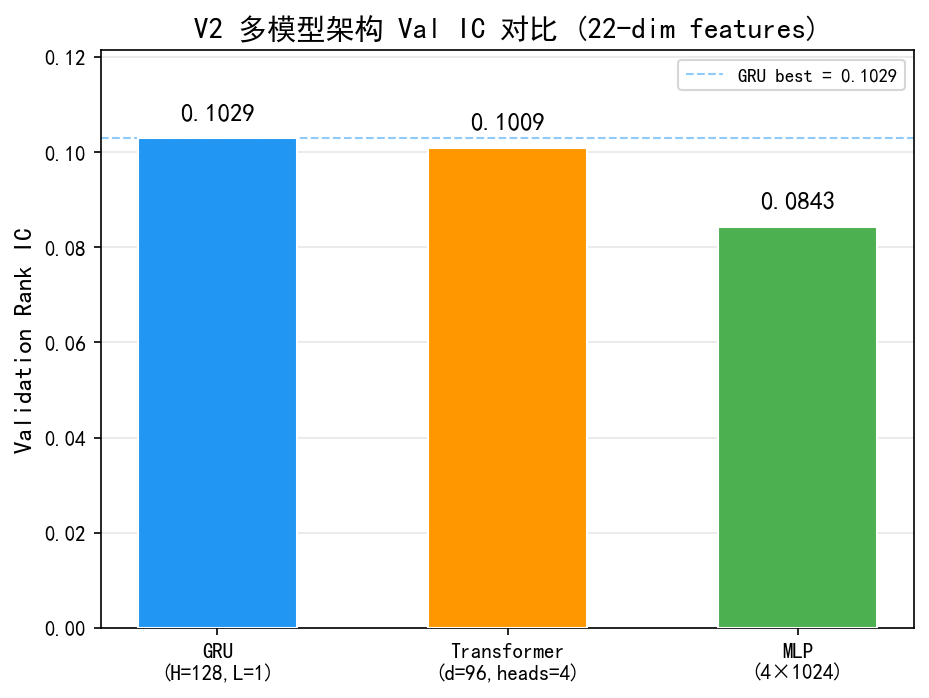
\includegraphics[width=0.75\textwidth]{fig1_model_comparison.png}
\caption{V2三模型验证IC对比}
\label{fig:v2_model}
\end{figure}

\subsection{交易策略设计与风控（V3）}

模型输出的是排序分数，如何将其转换为实际交易决策，涉及策略参数的选择和风险控制机制的设计。
V3在V2 GRU基础上，对N-K参数和多种减仓机制进行了系统性评估。

\subsubsection{Strategy B（动量止损）的确立}

在测试的多种减仓方案中，CSI300 5日收益率$<$-1.0\%时将仓位降至80\%的策略（Strategy B）
表现最优。其核心逻辑是\textbf{不对称风控}——宁可频繁减仓少赚，也要避免少数大跌幅对组合的毁灭性打击。

Strategy B有效的原因可以从三个层面理解：
\begin{enumerate}[leftmargin=*]
    \item \textbf{信号质量}：CSI300 5日收益率是直接的市场观测值，不是模型派生的二级指标，
          不受模型IC波动的影响。它测量的是市场整体的动量状态，而非个股层面的预测精度。
    \item \textbf{二元简洁性}：100\%/80\%的二值决策避免了连续映射的过拟合风险。
          二值”悬崖”创造了一个强行为信号：“市场要么正常，要么出问题了”。
          软化这个边界（连续减仓）会减弱保护效果而不增加收益（V3实验证实连续映射+5.56\% < 二值+6.85\%）。
    \item \textbf{跨regime鲁棒性}：在10窗口测试中，Strategy B在上半场（牛市）和下半场（震荡市）
          分别取得了+3.81\%和+0.50\%的增量收益，覆盖了8/10个最差交易日，
          弥补了116\%的沪深300差距。
\end{enumerate}

值得特别说明的是，V3进行了Variance Drag诊断，发现模型$\beta=1.41$——模型持仓放大了市场波动，
3个最差交易日吞噬了60天的利润。这进一步说明了风控机制的必要性：
\textbf{在信号薄弱的alpha模型上，风控的边际收益可能远超继续提升模型IC}。

\subsubsection{失败方案的诊断价值}

多种减仓方案被系统性地证伪，每个失败都对后续设计产生了影响：

\begin{itemize}[leftmargin=*]
    \item \textbf{波动率过滤（Strategy C/A+C）}：全部差于基线策略。根本原因在于
          低波动不等于抗跌——在系统性下跌中，所有股票一起跌，波动率排名不提供选股优势。
          同时波动率过滤也吃掉了GRU原有的选股信号。
    \item \textbf{Dispersion Defense（分数截面离散度）}：0胜3负7平。
          score\_std是非平稳的——其P95触发点完全集中在测试期尾部（最后10天），
          在10窗口回测中完全无效。对于10天的竞赛期，其价值为零。
    \item \textbf{Continuous Sizing（连续仓位映射）}：将二值仓位决策改为连续映射，
          所有线性/指数/波动率自适应方案均劣于二值阈值。
          二值悬崖是特征而非缺陷——软化边界减弱了动量止损的保护效果。
\end{itemize}

\textbf{关键认知}：在信号较弱的alpha模型上，简单二值规则优于复杂的连续/复合规则。
复杂性如果不能带来信息增益，只会引入额外的过拟合维度。

\begin{figure}[htbp]
\centering
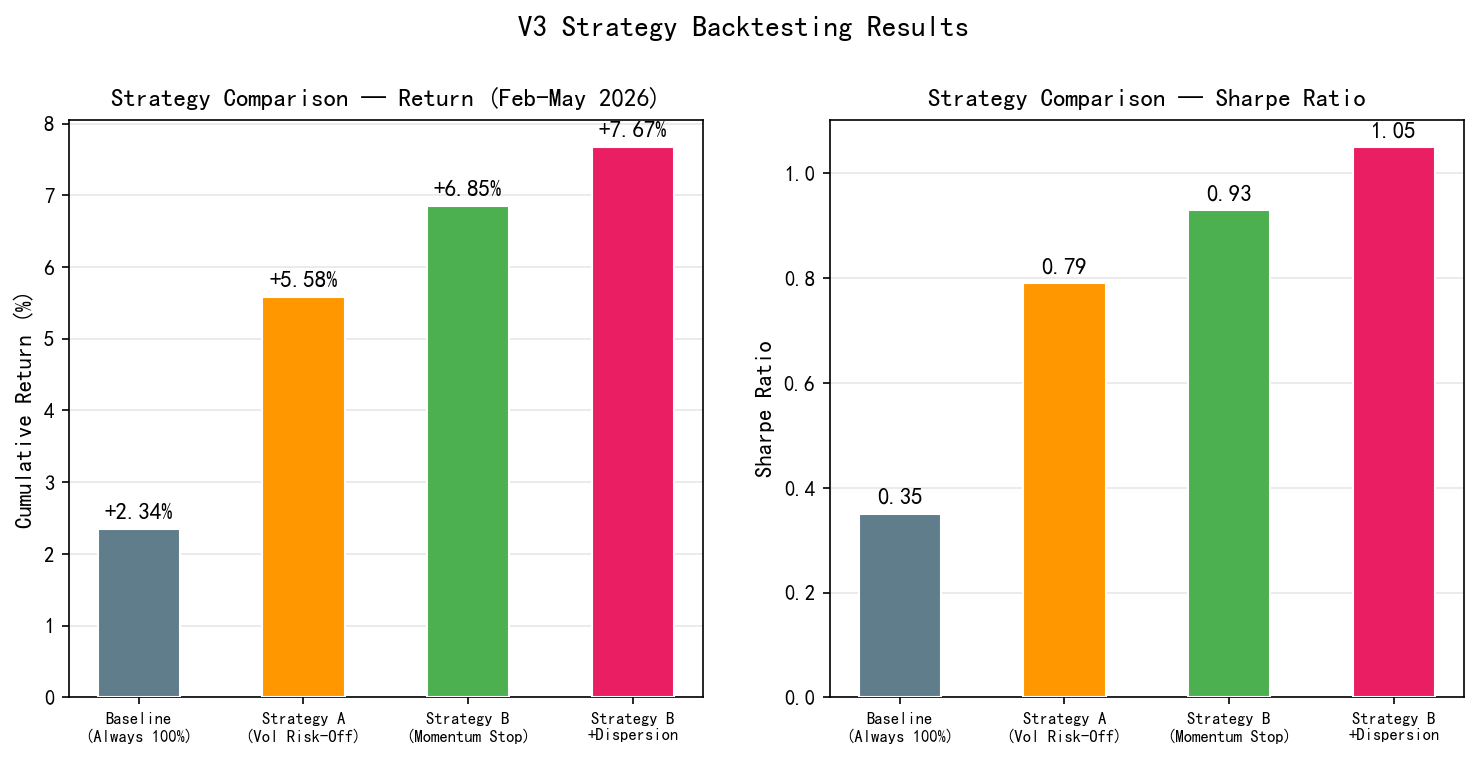
\includegraphics[width=0.75\textwidth]{fig3_strategy_comparison.png}
\caption{Strategy A/B/C对比}
\label{fig:v3_strategy}
\end{figure}

\subsection{多窗口集成的可行性探索（V4）}

\subsubsection{窗口对比实验}

V4探索了不同序列长度（$T=30,60,90$）的GRU是否捕捉不同周期的alpha信号，
以及多窗口融合能否提升稳健性。

\begin{table}[htbp]
\centering
\caption{不同序列长度的GRU模型IC对比}
\label{tab:v4_windows}
\begin{tabular}{cccc}
\toprule
指标 & $T=30$ & $T=60$ & $T=90$ \\
\midrule
Mean Rank IC & +0.0363 & \textbf{+0.0424} & +0.0430 \\
IC$>0$比例 & 61\% & 64\% & 65\% \\
IC相关性（vs $T{=}60$） & 0.962 & — & \textbf{0.997} \\
分数秩相关（vs $T{=}60$） & 0.845 & — & \textbf{0.9876} \\
\bottomrule
\end{tabular}
\end{table}

\subsubsection{放弃多窗口方向的三条理由}

\begin{enumerate}[leftmargin=*]
    \item \textbf{$T{=}90$完全冗余}：与$T{=}60$的IC相关性0.997、分数秩相关0.9876
          ——几乎是同一个模型。额外的30天历史没有提供新的信息维度。
    \item \textbf{$T{=}30$劣于且不互补}：单独IC 0.0363 $<$ 0.0424，
          IC相关性0.962——没有“30日 vs 60日”的regime分工。
          任何加权融合$w \cdot S_{30} + (1-w) \cdot S_{60}$的IC均低于$T{=}60$单独使用。
    \item \textbf{量化验证}：最优融合权重为$w=0$——即不使用$T{=}30$。
\end{enumerate}

这个结果说明：金融时序中，不同窗口长度的GRU模型学到的是高度相关的排序模式，
不会因为窗口长度不同而产生互补的alpha信号。这与“动量策略中短周期和长周期信号独立”
的直觉形成鲜明对比——GRU的门控机制使得模型能够自适应地利用窗口内的全部信息，
长窗口模型已经隐含包含了短窗口的历史。

\subsubsection{意外的副产品——KNN Proxy验证空间注意力}

在退出多窗口方向前，V4用一个低成本实验验证了空间注意力的可行性，
这成为后续V6架构升级的关键前置证据。

实验设计：使用固定截面特征（pct\_chg、amount、turnover\_rate）在测试期每天做KNN选择邻居，
对GRU分数做简单加权平均（$\alpha$为邻居权重的比例因子）。
如果邻居分数包含增量信息，则融合分数应优于纯GRU分数。

\begin{figure}[htbp]
\centering
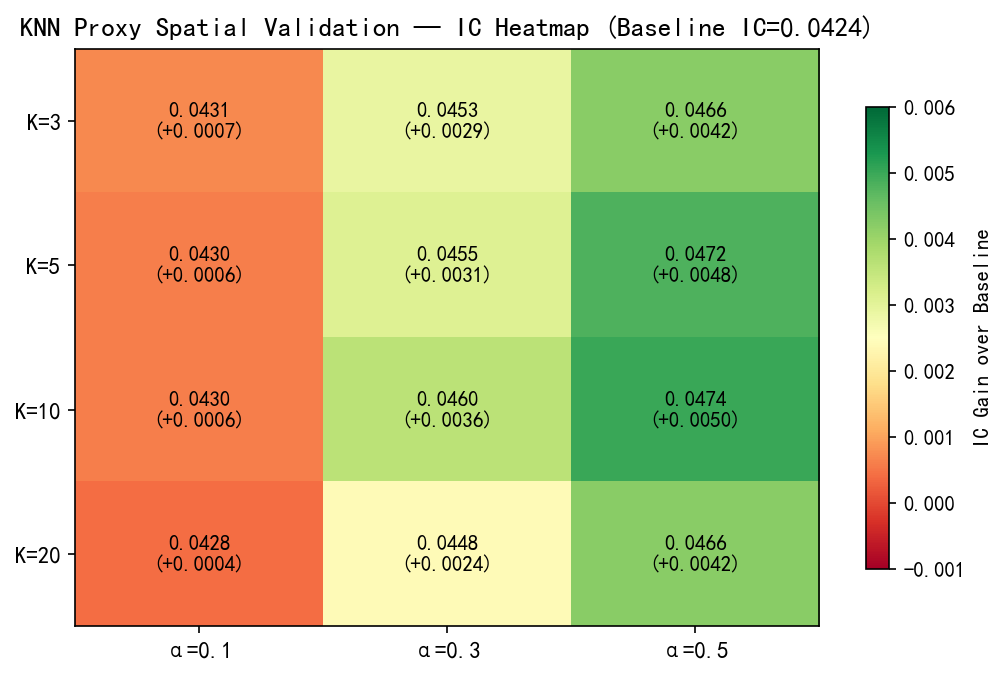
\includegraphics[width=0.7\textwidth]{fig5_knn_proxy_heatmap.png}
\caption{KNN Proxy K-$\alpha$ IC增益热力图}
\label{fig:v4_knn}
\end{figure}

结果如热力图所示：所有$(K, \alpha)$组合均正向，最佳增益为$K{=}10,\alpha{=}0.5$时的\textbf{+0.0049（+11.5\%）}。
增益来自日IC的量级提升而非方向性提升（IC$>0$比例不变），
说明邻居信息起到了非参数去噪的作用——
对相似股票取平均，抹掉个股噪声，但不改变信号方向。

这一发现的意义在于：\textbf{GRU的隐状态没有完全提取截面上的股票间相关信息}，
邻居股票的分数包含可被KNN这类简单线性聚合捕捉的增量信息。
如果可学习的注意力机制能自动发现比KNN更优的邻居选择策略，有望获得超越+0.0049的增益。

\subsection{预处理体系重构：最大的单次突破（V5）}

V5是整个迭代过程中单次IC提升最大的版本，但其核心贡献不是新增了什么，而是\textbf{修复了一个隐藏的关键缺陷}。

\subsubsection{缺陷根因：截面特征全部失效}

在V1--V4的22维特征管线中，4个截面特征——$\text{rank}(\text{pct\_chg})$、
$\text{rank}(\text{amount})$、$\text{rank}(\text{turnover\_rate})$、
$\text{pct\_chg} - \text{CSI300\_ret}$——先被tile到60个时间步，
再经受per-window Z-score归一化。问题是：截面值在一个时间步上的所有股票间是常数，
在时间轴上每个时间步也是同一组数值。Z-score归一化后，每个特征的60个时间步均值相同，
标准差为零——归一化后\textbf{全部退化为零向量}。

这意味着模型实际只在$22-4=18$维有效特征上训练了V1--V4的所有版本。
V2的0.1029和V3的+6.85\%回测收益，都是在\textbf{缺失截面信息}的情况下取得的。

\subsubsection{两阶段归一化}

V5的修复方案将归一化拆分为两条独立路径：

\begin{itemize}[leftmargin=*]
    \item \textbf{时序特征（per-window Z-score）}：量价和技术指标沿时间轴独立标准化，
          不同时间步的均值和标准差互不依赖
    \item \textbf{截面特征（per-date Z-score）}：截面排名和估值指标先在当日的股票横截面上标准化，
          \textbf{再}tile到时间维度。这个顺序是关键——先截面标准化保留股票间的相对关系，
          再扩展到时间轴，确保每个时间步上的截面值具有区分度
\end{itemize}

\subsubsection{伴随改进与效果}

除归一化修复外，V5还进行了多项预处理增强：新增5维特征（vwap\_gap机构活动信号、
$\text{rank}(\text{pe})$、$\text{rank}(\text{pb})$、$\text{rank}(\text{circ\_mv})$），
特征维度从22维升至26维；对vol、amount、total\_mv做log1p变换压缩长尾分布；
对所有时序特征做1\%/99\%分位winsorization抑制异常日；
PE限制在[0.1, 500]、PB限制在[0.1, 50]。

\begin{table}[htbp]
\centering
\caption{V5预处理修复效果}
\label{tab:v5_improvement}
\begin{tabular}{lcc}
\toprule
版本 & 预处理 & 验证IC \\
\midrule
v5.1 & 仅修复归一化bug，无额外预处理 & 0.1030 \\
\textbf{v5.2} & \textbf{修复bug + log1p + winsor + PE/PB clip + 新特征} & \textbf{0.1114} \\
\midrule
提升 & & \textbf{+8.2\%} \\
\bottomrule
\end{tabular}
\end{table}

V5贡献了\textbf{+8.2\%}的验证IC提升——这一幅度远超后续所有架构改进的边际增益
（V6的空间注意力仅贡献+1.8\%）。一个bug的修复和一个合理的归一化设计，
其价值超过新架构、新特征、新损失函数的总和。
\textbf{在金融数据上，特征工程的重要性远大于模型架构}——这是路线A最核心的经验。

\subsection{空间注意力机制的设计与修正（V6）}

V4的KNN Proxy实验已经证明：利用截面上的“相似股票”信息可以增强排序精度（+11.5\% IC增益）。
V6的目标是将这一思想转化为可端到端学习的注意力模块。

\subsubsection{V1失败版：缺失瓶颈设计}

初版实现使用$d_{\text{proj}}=128$（等于隐层维度）的Q/K/V投影，
Top-K稀疏化后残差连接。结果：验证IC从0.1114降至0.1086（\textbf{-2.5\%}），
没有复现KNN proxy的增益。

失败根因在事后与原始设计文档（\texttt{SPATIAL\_ATTENTION\_PLAN.md}）对比时被发现，
存在三个关键偏差：

\begin{table}[htbp]
\centering
\caption{V6 V1空间注意力失败诊断}
\label{tab:v6_v1_diagnosis}
\begin{tabular}{lccp{4cm}}
\toprule
设计维度 & 原始计划 & V1实现 & 后果 \\
\midrule
Q/K投影维度 & \textbf{$d{=}32$}（瓶颈） & $d{=}128$（=hidden\_size） & 128维全空间计算相似度，无关维度淹没信号 \\
融合方式 & concat/gated/residual扫描 & 仅residual & 未测最优融合 \\
投影层 & Linear(32$\to$128) & 无投影 & 噪声等权注入hidden state \\
\bottomrule
\end{tabular}
\end{table}

\textbf{核心错误}：$d < d_{\text{model}}$是注意力瓶颈设计的核心原则。
当$d=128$时，Q/K投影近乎恒等映射，
相似度$\approx \mathbf{h} \cdot \mathbf{h}^\top$，
模型无法学习到有意义的邻居关系。
KNN Proxy之所以能成功，是因为它用\textbf{固定截面特征}选择邻居——
这是非参数去噪，而非learnable attention。
将Q/K投影到32维瓶颈空间，迫使模型选择对“找邻居”最关键的维度。

\subsubsection{V2修正版：成功的关键}

修正措施：$d_{\text{proj}}=32$ 瓶颈 + self-exclude
（$\text{sim}[i,i]=-\infty$替代V1的手动topk+remove）+ 三种融合方式扫描 +
Linear(32$\to$128)投影。

\begin{table}[htbp]
\centering
\caption{V6 V2空间注意力融合方式对比}
\label{tab:v6_fusion}
\begin{tabular}{lcc}
\toprule
融合方式 & 验证IC & vs Baseline \\
\midrule
concat & 0.1126 & +1.1\% \\
gated & 0.1122 & +0.7\% \\
\textbf{residual} & \textbf{0.1131} & \textbf{+1.5\%} \\
\bottomrule
\end{tabular}
\end{table}

三种融合方式全部超越基线模型，验证了$d=32$ 瓶颈是决定性因素。
进一步K值扫描发现，residual融合在$K=5$时达到最优IC 0.1134（concat+0.1134、residual+0.1124），
而全规模$N_{\text{sample}}=2048$时IC降至0.1099——更多股票引入更多噪声邻居，
降低了空间注意力的信噪比，$N_{\text{sample}}=1024$是最优点。

\begin{figure}[htbp]
\centering
\begin{subfigure}{0.48\textwidth}
    \centering
    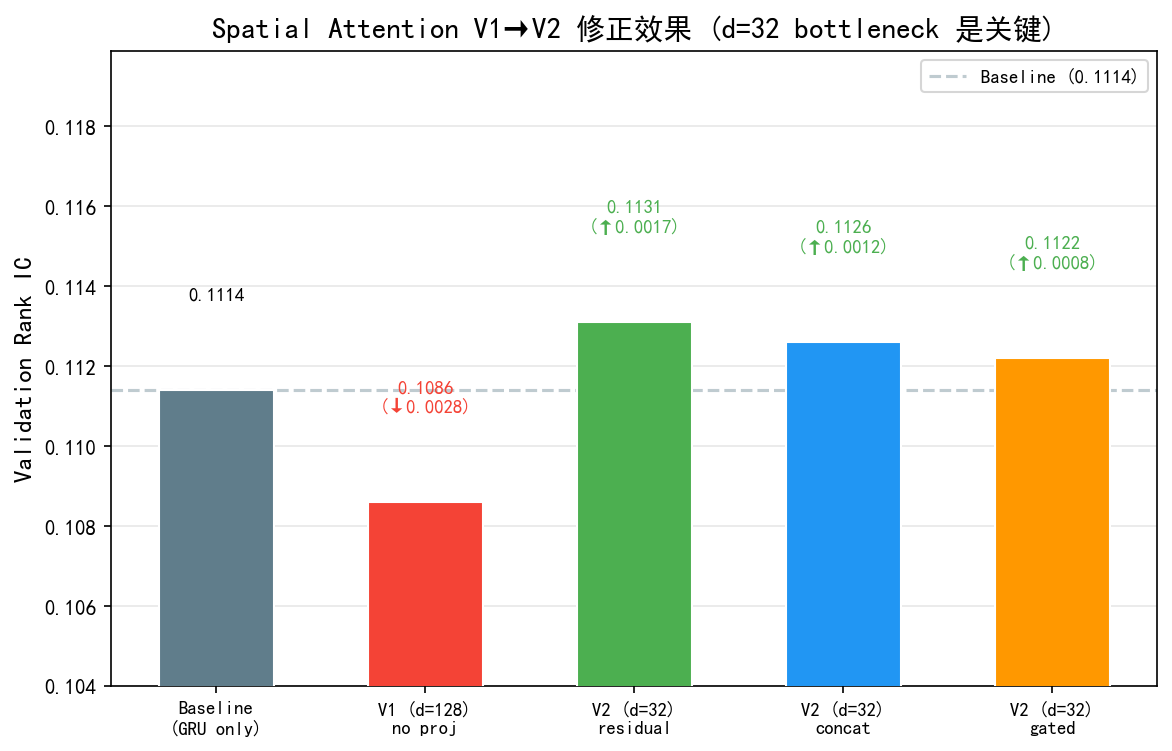
\includegraphics[width=\textwidth]{fig6_spatial_v1_v2.png}
    \caption{V1$\to$V2修正效果}
    \label{fig:v6_spatial}
\end{subfigure}
\hfill
\begin{subfigure}{0.48\textwidth}
    \centering
    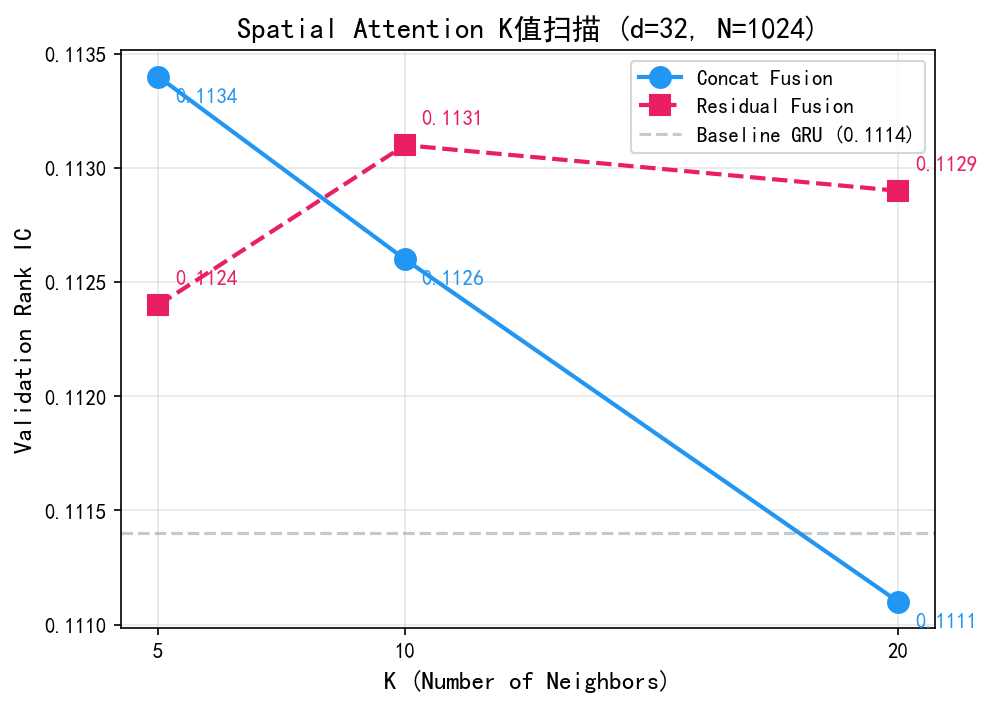
\includegraphics[width=\textwidth]{fig7_k_sweep.png}
    \caption{K值扫描}
    \label{fig:v6_k}
\end{subfigure}
\caption{空间注意力机制的设计迭代}
\end{figure}

\subsection{标签修正与最优模型确立（V7）}

\subsubsection{T+5标签的虚假繁荣}

V5--V6使用T+5累计收益率作为标签（$\sum_{k=1}^{5} \text{pct\_chg}[t+k]$），
验证IC达到0.111--0.113的亮眼成绩。但V6的测试期诊断揭示了一个严重问题：

\begin{table}[htbp]
\centering
\caption{V6模型在测试期的预测能力——标签错配}
\label{tab:v6_label_mismatch}
\begin{tabular}{lcc}
\toprule
预测标的 & Test IC & IC$>0$比例 \\
\midrule
T+1收益率（模型实际在预测的） & \textbf{0.053} & 67.6\% \\
T+5收益率（模型被训练预测的） & \textbf{0.010} & \textbf{42.6\%} \\
\bottomrule
\end{tabular}
\end{table}

T+5的测试IC 0.010比随机还差（IC$>0$仅42.6\%）。根因是训练期的动量延续效应：
2019--2024年间T+1动量与T+5累计收益高度相关，模型只需学会T+1动量模式就能在T+5标签上拿高分；
2026年动量断裂后，T+1$\neq$T+5，真相暴露。

\textbf{决策：回归T+1标签。}虽然验证IC从0.113“降低”至0.106，
但这是诚实的信号——模型不再依赖动量溢价提供的虚假相关性。
从Val→Test的IC衰减也从T+5的$0.113\to 0.010$（-91\%）
改善为T+1的$0.106\to 0.048$（-55\%，含正常的OOS衰减）。

\subsubsection{重训结果与空间注意力的放大器效应}

\begin{table}[htbp]
\centering
\caption{V7 T+1标签重训结果}
\label{tab:v7_retrain}
\begin{tabular}{lccc}
\toprule
模型 & 标签 & 验证IC & 参数量 \\
\midrule
v5 GRU & T+5 & 0.1114 & 68,225 \\
v7 GRU & T+1 & 0.1023 & 68,225 \\
\textbf{v7 Spatial} & \textbf{T+1} & \textbf{0.1062} & \textbf{82,561} \\
\bottomrule
\end{tabular}
\end{table}

T+1的验证IC天然低于T+5——单日噪声远大于5日平滑——但Spatial在T+1上仍有效（+0.0039 vs GRU），
且收敛更稳定（30 epoch vs 14 epoch）。更关键的是，
空间注意力在T+1标签上的放大器效应远远强于在T+5标签上：
在T+5上，V6 Spatial的N=5 K=3回测仅比基线模型高+0.07\%；
在T+1上，V7 Spatial同等配置的回测比GRU 基线模型高\textbf{4.5倍}（+15.45\% vs +3.43\%）。
\textbf{正确的标签是架构发挥威力的前提。}

\subsubsection{N-K参数扫描}

对V7 Spatial在600股测试集上的全参数扫描确认了N=5, K=3为最优配置：

\begin{figure}[htbp]
\centering
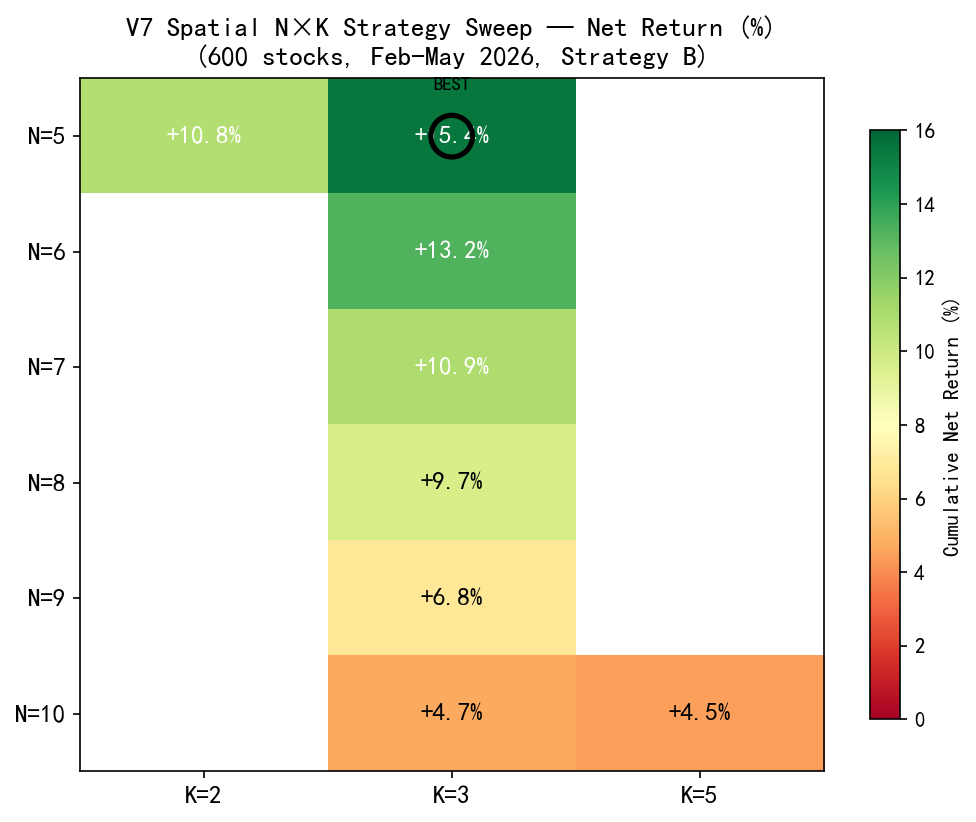
\includegraphics[width=0.7\textwidth]{fig9_nk_sweep_heatmap.png}
\caption{V7 Spatial N$\times$K扫参热力图}
\label{fig:v7_nk}
\end{figure}

关键发现：每增持1只股票，收益下降1.2--2.9\%——模型的alpha高度集中在前5名，
第6--10名的信号迅速稀释。所有N值下K=3均为最优，说明适度的换手（60\%）在捕捉新信号
和承受交易成本之间取得了最佳平衡。

\subsection{失败的扩展尝试（V8--V9）}

\subsubsection{V8：特征扩展与行业信息注入}

V8尝试从三个方向寻找增量：新特征（资金流+流动性+偏度）、新损失函数、行业嵌入。

\textbf{为什么没有从一开始就使用资金流数据？}
在设计V1--V7的特征管线时，有意识地将资金流数据排除在外，基于两点考虑：
第一，资金流向数据本质上是\textbf{量价数据的衍生指标}——大单买入/卖出、主力净流入等
都是从成交明细中聚合而来，其信息已隐含在量价序列中；
第二，A股市场存在\textbf{主力伪造资金流向}的现象——通过拆单、对倒等手法，
大资金可以制造“主力净流入”的虚假信号诱导散户跟风。
课程提供的资金流数据共19个维度，涵盖了按大/中/小单、机构/散户分类的净买卖量和净买卖额，
但其中隐含的博弈关系极其复杂。在V1--V7阶段，
策略是\textbf{先让模型从相对干净的26维量价+技术+截面特征中提取信号}，
待基线稳定后再引入资金流做增量验证。

V8的实验结果部分印证了这一审慎判断。

\textbf{方向1：特征扩展（31维 + 行业Embedding）。}
基于IC诊断（2024--2025年，338天，600股），从30+候选特征中选出最优5个。
其中资金流集中度（mf\_flow\_hhi，IC=+0.046）和流动性指标（amihud\_20，IC=+0.028）
的单因子IC表现不错。同时注入111个行业的8维Embedding到Head MLP。

结果：验证IC从0.1062降至0.1037，回测收益暴跌64\%。

失败根因可以归结为两个层面：
\begin{enumerate}[leftmargin=*]
    \item \textbf{资金流数据与GRU时序模式的分布不兼容}。资金流数据来自完全不同的数据源（19列），
          其统计特性（分布形态、时间自相关、截面方差）与OHLCV迥异。
          GRU在60天窗口中同时处理价格序列和资金流序列时，两域的梯度相互干扰——
          价格域学到的时序模式（如突破、回调）被资金流的噪声梯度打乱。
          这是“多源数据融合”的经典陷阱：直接拼接不等同于有效融合。
    \item \textbf{行业Embedding注入位置过浅}。行业信息在GRU处理完60天时序后才流入（concat到Head MLP），
          对GRU内部的时序处理毫无影响。$\lambda{=}0.1$的门控加成在注意力量级（$\sim$2）中几乎不可见，
          且行业是静态标签——模型可能学会给某行业系统性高分/低分，这不利于横截面排序（排序需要区分同行业内股票的相对强弱）。
\end{enumerate}

\textbf{方向2：损失函数对比。}
在完全相同条件下训练三个模型，Weighted ListMLE（$\alpha{=}0.9$）
的验证IC为-0.067——指数衰减权重使模型在$N{=}1024$样本中只认真学前30个位置的排序，
剩余97\%股票梯度为零，全局排序崩溃。
LambdaRank的验证IC仅为0.007——其DCG gain函数将所有labels平移为非负，
扭曲了连续收益率之间的相对关系。ListMLE是唯一有效的选择。

\textbf{方向3：减仓指标优化。}
对15个市场特征与“5日跌$>3\%$”的相关性扫描发现，
最大相关性仅为+0.079——没有任何指标能可靠预测短期暴跌。
CSI5d $<$ -1\%的简单规则，虽然缺乏理论优雅性，但它在2026年实际触发的那几天恰好是真跌日。
这不是设计的结果，但在缺少更优替代方案的情况下，它是经验上最稳健的选择。

\subsubsection{V9：售卖模型与微调}

V9进行了两个方向的前提验证实验。

\textbf{售卖模型}：独立训练一个模型专门优化“卖谁”的决策，
使用regime-conditional volatility做卖单排序（熊市卖高波动、牛市卖低波动）。
遍历$\lambda \in [0, 0.5, 1.0, 2.0, 3.0, 5.0, 10.0]$，所有变体的收益均不高于基线。
\textbf{售卖模型的前提被证伪}：v7的排序分数本身已是足够强的卖单信号，
叠加vol指标只会劣化。

\begin{figure}[htbp]
\centering
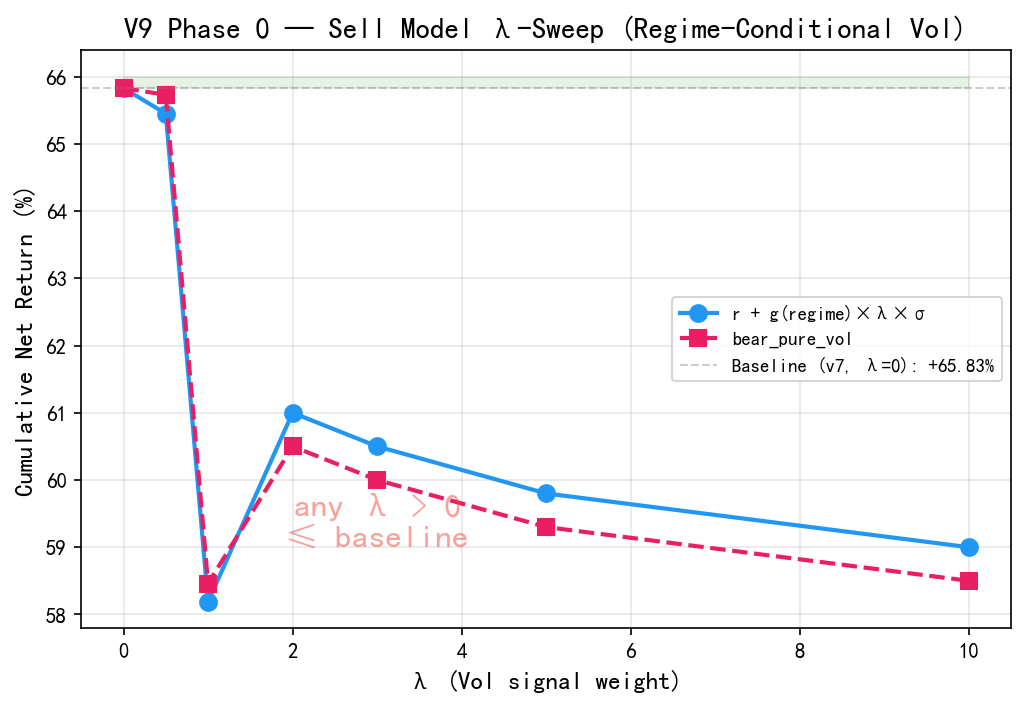
\includegraphics[width=0.6\textwidth]{fig15_lambda_sweep.png}
\caption{V9 $\lambda$扫描——任何$\lambda>0$均不高于基线}
\label{fig:v9_lambda}
\end{figure}

\textbf{微调}：在2025年验证集上fine-tune v7模型20个epoch，
ListMLE loss仅从6030降至6025（0.08\%改善）。
因为v7已通过early stopping在验证集上选出了最优checkpoint，额外微调无增益。

\textbf{Jan 2026效应分析}：V7 Spatial的全周期回测中，1月贡献了全周期收益的85.7\%。
Alpha/Beta分解显示1月收益的88\%来自真实alpha（选股能力），仅12\%来自市场beta放大。
但4月后IC跌至不显著水平（-0.007，p=0.490），
模型在regime切换后失效——训练期（2019--2024）学到的模式在2026年4月的政策驱动型V型反弹中不再有效。

\begin{figure}[htbp]
\centering
\begin{subfigure}{0.48\textwidth}
    \centering
    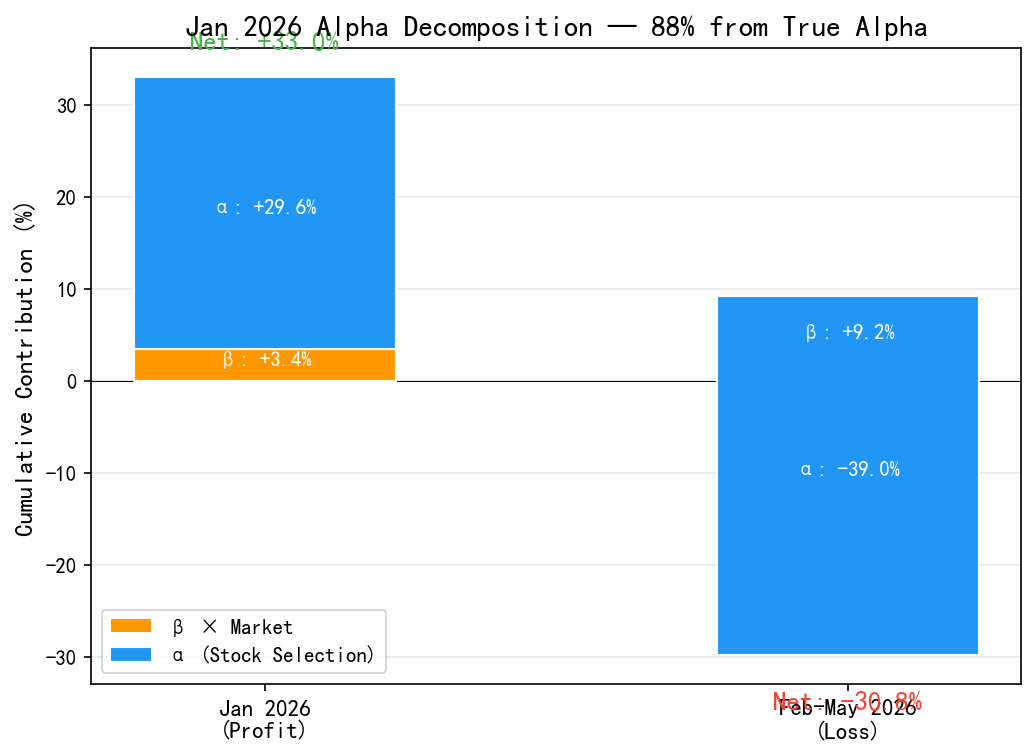
\includegraphics[width=\textwidth]{fig16_jan_decomposition.png}
    \caption{Jan效应Alpha/Beta分解}
\end{subfigure}
\hfill
\begin{subfigure}{0.48\textwidth}
    \centering
    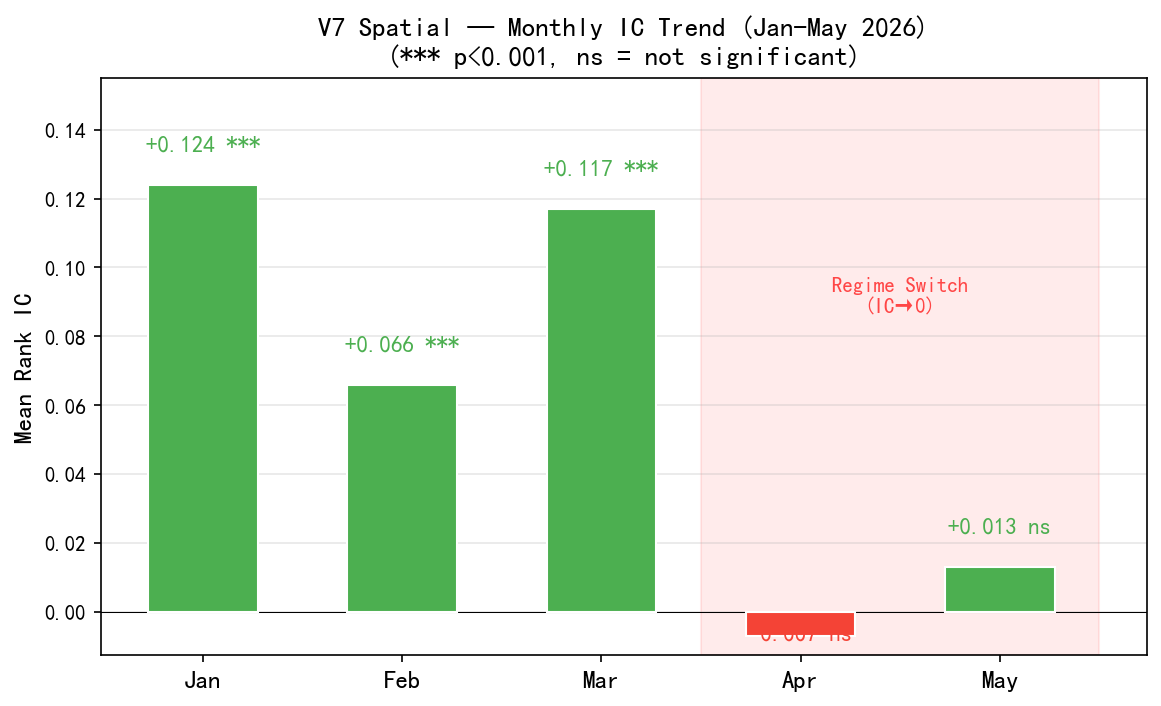
\includegraphics[width=\textwidth]{fig17_monthly_ic_trend.png}
    \caption{月度IC趋势——4月后失效}
\end{subfigure}
\caption{V9 效应诊断}
\end{figure}

\subsection{版本迭代总结}

表\ref{tab:version_overview}汇总了V1至V9九个版本的核心变化与验证集表现。

\begin{table}[htbp]
\centering
\caption{路线A版本迭代总览}
\label{tab:version_overview}
\small
\begin{tabular}{cclc}
\toprule
版本 \& 核心工作 \& 关键决策 \& 验证IC \\
\midrule
V1 \& GRU基线搜索 \& 确定\$T{=}60,H{=}128,L{=}1\$为最优超参 \& 0.1042 \\
V2 \& 多模型对比+特征扩展 \& GRU优于TF/MLP；特征从10维扩至22维 \& 0.1029 \\
V3 \& 策略回测+止损机制 \& Strategy B（动量止损）确立 \& --- \\
V4 \& 多窗口集成探索 \& \$T{=}90\$与\$T{=}60\$高度冗余，放弃多窗口 \& --- \\
V5 \& 截面特征修复 \& 两阶段归一化\to IC +8.2\% \& 0.1114 \\
V6 \& 空间注意力 \& \$d{=}32\$瓶颈设计是关键 \& 0.1134 \\
V7 \& T+1标签修正 \& 从T+5回归T+1，诚实面对可预测性 \& \textbf{0.1062} \\
V8 \& 特征扩展+行业嵌入 \& 多源数据冲突导致全面退化 \& 0.1037 \\
V9 \& 售卖模型+微调 \& 均无增量，前提被证伪 \& --- \\
\bottomrule
\end{tabular}
\end{table}

九个版本的迭代中，超过一半的尝试以失败告终。
V5的预处理修复贡献了最大的单次验证IC提升（+8.2\%），远超任何架构改进；
V6的空间注意力在正确设计下取得了+1.8\%的增益；
V7通过标签修正（T+5\to T+1）获得了诚实且可泛化的信号。
V8--V9的失败则排除了资金流特征直拼和售卖模型两个方向。
从V1的0.1042到V7的0.1062，验证IC的绝对提升不到0.002---
这个看似微小的进步背后，是9个版本、14个主要尝试方向、超过一半失败率的真实探索过程。

\subsection{统一回测与信号质量分析}

本节在统一回测框架（2026年1月5日至5月29日，94个交易日，净值成本模型，Strategy B，
N=5 K=3）下汇总路线A各模型的回测表现。

\subsubsection{信号质量对比}

表\ref{tab:routeA_ic_summary}汇总了路线A三个模型在统一测试期上的Rank IC表现。

\begin{table}[htbp]
\centering
\caption{路线A信号质量汇总（统一测试期，94天）}
\label{tab:routeA_ic_summary}
\begin{tabular}{lcccc}
\toprule
模型 & Mean Rank IC & IC Std & ICIR & IC$>0$比例 \\
\midrule
V6 Spatial (T+5) & 0.062 & 0.157 & 0.39 & 69.5\% \\
V7 GRU (T+1) & 0.069 & 0.165 & 0.42 & 65.3\% \\
V7 Spatial (T+1) & 0.074 & 0.159 & 0.47 & 67.4\% \\
\bottomrule
\end{tabular}
\end{table}

三个模型的Rank IC均在0.06--0.07之间，ICIR在0.39--0.47——信号方向性的稳定性尚可，
但量级上属于“薄信号”范畴（单日IC标准差约为均值的2--3倍）。

\subsubsection{日度IC时序分析}

图\ref{fig:daily_ic}展示了三个模型的日度Rank IC叠加时序。
三个模型的IC走势高度同步——IC相关性超过0.95——说明它们捕捉的是同一个底层信号维度，
架构差异（GRU vs GRU+Spatial）仅改变了信号的量级，未改变信号的方向模式。

\begin{figure}[htbp]
\centering
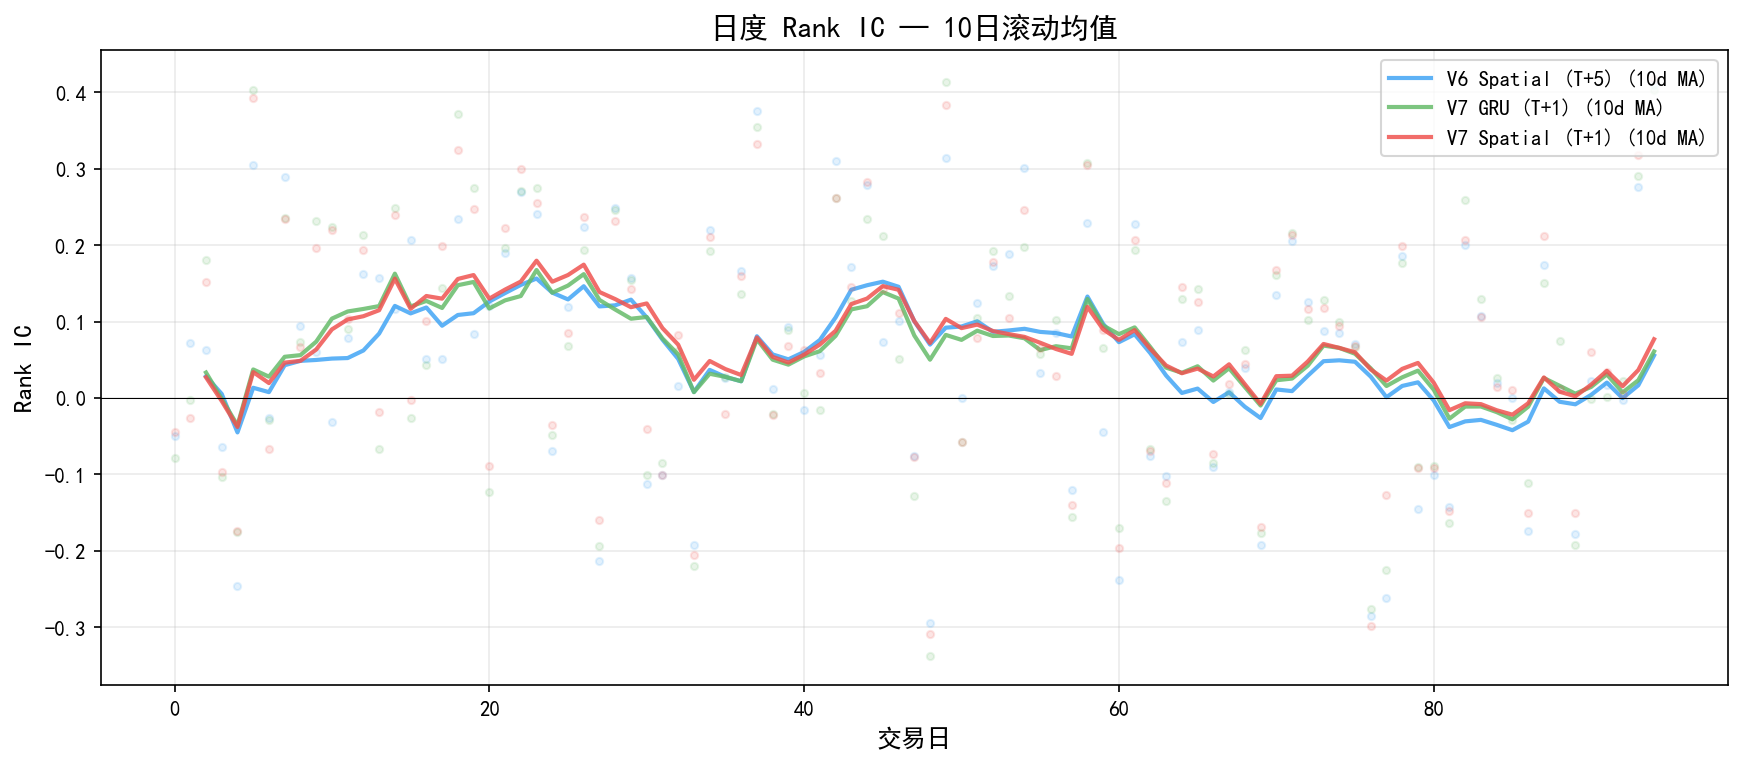
\includegraphics[width=\textwidth]{fig_daily_ic.png}
\caption{日度Rank IC时序（10日滚动均线）}
\label{fig:daily_ic}
\end{figure}

\subsubsection{月度IC稳定性}

图\ref{fig:monthly_ic_box}的月度箱线图揭示了信号质量的时间衰减模式：
1--3月IC维持在正值区间（中位数0.05--0.10），4--5月IC迅速衰减至零附近。
这与2026年4月沪深300暴涨+8.03\%的政策驱动行情高度吻合——
市场驱动力从因子分化切换为Beta驱动，横截面排序模型的预测能力系统性下降。

\begin{figure}[htbp]
\centering
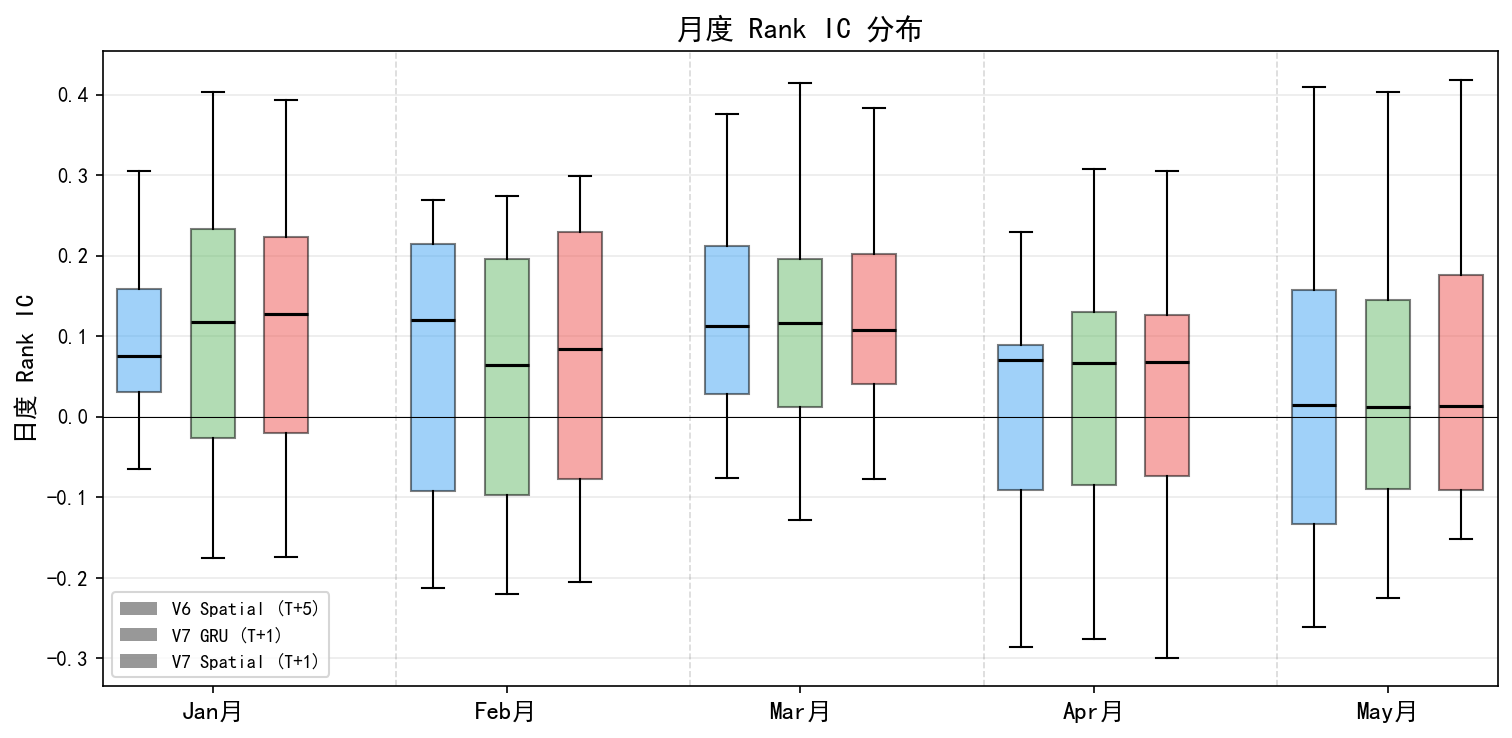
\includegraphics[width=\textwidth]{fig_monthly_ic_box.png}
\caption{月度Rank IC分布箱线图}
\label{fig:monthly_ic_box}
\end{figure}

\subsection{版本迭代核心经验}

九个版本的迭代过程中，超过一半的尝试（8/14）以失败告终。表\ref{tab:failures}汇总了重要的失败案例及其教训。

\begin{table}[htbp]
\centering
\caption{重要失败尝试与教训}
\label{tab:failures}
\small
\begin{tabular}{llp{5cm}}
\toprule
尝试 & 版本 & 教训 \\
\midrule
T+5标签 & V5--V6 & 标签必须与实际预测能力匹配；验证IC高不代表预测能力真实 \\
V1空间注意力（$d{=}128$） & V6 & $d < d_{\text{model}}$是注意力瓶颈设计核心原则 \\
多窗口集成 & V4 & 不同窗口的GRU不提供互补信息（$T{=}60$与$T{=}90$秩相关0.99） \\
资金流特征扩展 & V8 & 不同数据源应先经独立编码再融合，不宜直接拼入统一时序 \\
行业Embedding & V8 & 静态分类特征应在输入级注入GRU，而非事后concat到Head \\
售卖模型 & V9 & regime-conditional vol对卖决策零增量 \\
Fine-tuning & V9 & early stopping已选出最优checkpoint，微调无增益 \\
Dispersion Defense & V3 & 分数截面离散度非平稳，信号集中在尾部——竞赛期价值为零 \\
连续仓位映射 & V3 & 二值悬崖是特征而非缺陷——软化边界减弱动量止损的保护效果 \\
\bottomrule
\end{tabular}
\end{table}

\textbf{最核心的经验}：\textbf{特征工程 $\gg$ 模型架构}。
V5的bug修复+预处理贡献了+8.2\%的验证IC提升，
而V6的空间注意力（路线A最成功的架构改进）仅贡献+1.8\%。
在金融数据上，好的数据远比复杂的模型重要。
其次，\textbf{标签诚实性是不可妥协的}——T+5标签的“高分”经不起测试期检验，
回归T+1虽然验证IC更低，但预测能力更真实可信。
最后，\textbf{大部分尝试都会失败}——快速识别、果断放弃、从每个失败中提取一条明确的教训，
是比坚持无效方向更重要的能力。

% ═══════════════════════════════════════════════════════════
\section{路线B：价格预测路线的探索（吴同学）}
% ═══════════════════════════════════════════════════════════

\subsection{技术路线总览}

路线B采用与传统时间序列预测更接近的范式：使用CNN-LSTM模型预测次日收盘价，
然后通过$\hat{r}_{t+1} = \hat{p}_{t+1} / p_t - 1$反算预期收益率，按预期收益率排序选股。

与路线A的本质区别在于优化目标：
\begin{itemize}[leftmargin=*]
    \item 路线A优化\emph{相对排序}（“A比B好”），用ListMLE直接最大化排序概率
    \item 路线B优化\emph{绝对价格}（“明天价格是多少”），用MSE最小化预测误差
\end{itemize}

路线B的实验历程经历了三个阶段，每个阶段的设计由前一阶段的问题驱动，
整个过程体现了“数据量是深度学习效果的第一约束”这一核心认知。

\subsection{模型架构：CNN-LSTM}

路线B的模型架构如表\ref{tab:wu_arch}所示，其设计哲学是\emph{用深度换取特征简约}：
仅使用1维输入（归一化后收盘价），但通过CNN提取局部价格形态，LSTM建模时序依赖。

\begin{table}[htbp]
\centering
\caption{CNN-LSTM架构参数}
\label{tab:wu_arch}
\begin{tabular}{lrl}
\toprule
层级 & 参数 & 参数量 \\
\midrule
Conv1d($1\to64$, $k=3$) & ReLU & 192 \\
Conv1d($64\to64$, $k=3$) & ReLU & 8,256 \\
Conv1d($64\to64$, $k=3$) & MaxPool1d & 8,256 \\
LSTM($64\to256$)$\times$2层 & — & 856,064 \\
Linear($256\to1$) & — & 257 \\
\midrule
\textbf{合计} & & \textbf{864,769} \\
\bottomrule
\end{tabular}
\end{table}

架构的三个关键设计要点：

\begin{enumerate}[leftmargin=*]
    \item \textbf{CNN作为特征提取器}：三层Conv1d($k=3$)负责从原始价格序列中学习短期的局部价格形态
          （如突破、回调、盘整等），MaxPooling起降噪作用。
          CNN部分仅贡献约8K参数（占总量的$\sim$1\%），但其存在使IC提升了\textbf{3倍以上}
          （纯LSTM最佳IC=0.058 vs CNN-LSTM=0.226，单年实验）。
    \item \textbf{双层LSTM(256)作为时序建模器}：LSTM承担了91.5\%的参数量（791K），
          负责从CNN提取的局部特征中学习长期时序依赖。
    \item \textbf{极简输入}：仅使用1维归一化收盘价，不走多特征融合路线。
          这一设计的隐含假设是：如果模型架构足够深（865K参数），
          它可以自动从价格序列中发现有效的交易信号，而不需要人工构造技术指标。
\end{enumerate}

\subsection{归一化方案的系统性对比}

路线B投入了大量精力对比两种收盘价归一化方案，这一对比构成了其最重要的方法论贡献。
两种方案在原理和效果上的差异，与路线A的两阶段归一化修复形成了跨路线的呼应。

\subsubsection{方案一：因果累积Max-Min归一化}

对每只股票独立做因果累积的Min-Max缩放：
\begin{equation}
\text{scaled}[i] = \frac{\text{close}[i] - \min_{j \le i}(\text{close}[j])}
                         {\max_{j \le i}(\text{close}[j]) - \min_{j \le i}(\text{close}[j])}
\end{equation}

核心特性与路线A的归一化原则高度一致：
\begin{itemize}[leftmargin=*]
    \item \textbf{按股票独立}：消除绝对价格差异，无需对1元股和100元股做同一套缩放
    \item \textbf{因果累积}：只用截至当日的历史极值，无未来信息泄漏
    \item \textbf{噪声注入}：训练集施加乘性高斯噪声$\mathcal{N}(0, 0.03)$，增强鲁棒性
\end{itemize}

\subsubsection{方案二：全局Sigmoid归一化的系统性失效}

Sigmoid方案使用全局参数$\text{start}=0$和$\text{end}=500$将全市场股票映射到$(0,1)$区间。
该方案在A股市场完全失效，源于三个不可调和的设计缺陷：

\begin{enumerate}[leftmargin=*]
    \item \textbf{分布错位}：A股市场93.38\%的股票收盘价$\le$52元，
          全部落在Sigmoid左侧平缓区（梯度$\approx$0），不同股票间的缩放值几乎不可区分。
    \item \textbf{全局参数不灵活}：单一参数无法同时适配1元低价股和100元以上高价股。
    \item \textbf{极端值拖垮分辨率}：全市场最高价达2,601元，迫使$\text{end}=500$远离主流股价范围，
          绝大部分股票被压缩到极窄区间。
\end{enumerate}

\begin{figure}[htbp]
\centering
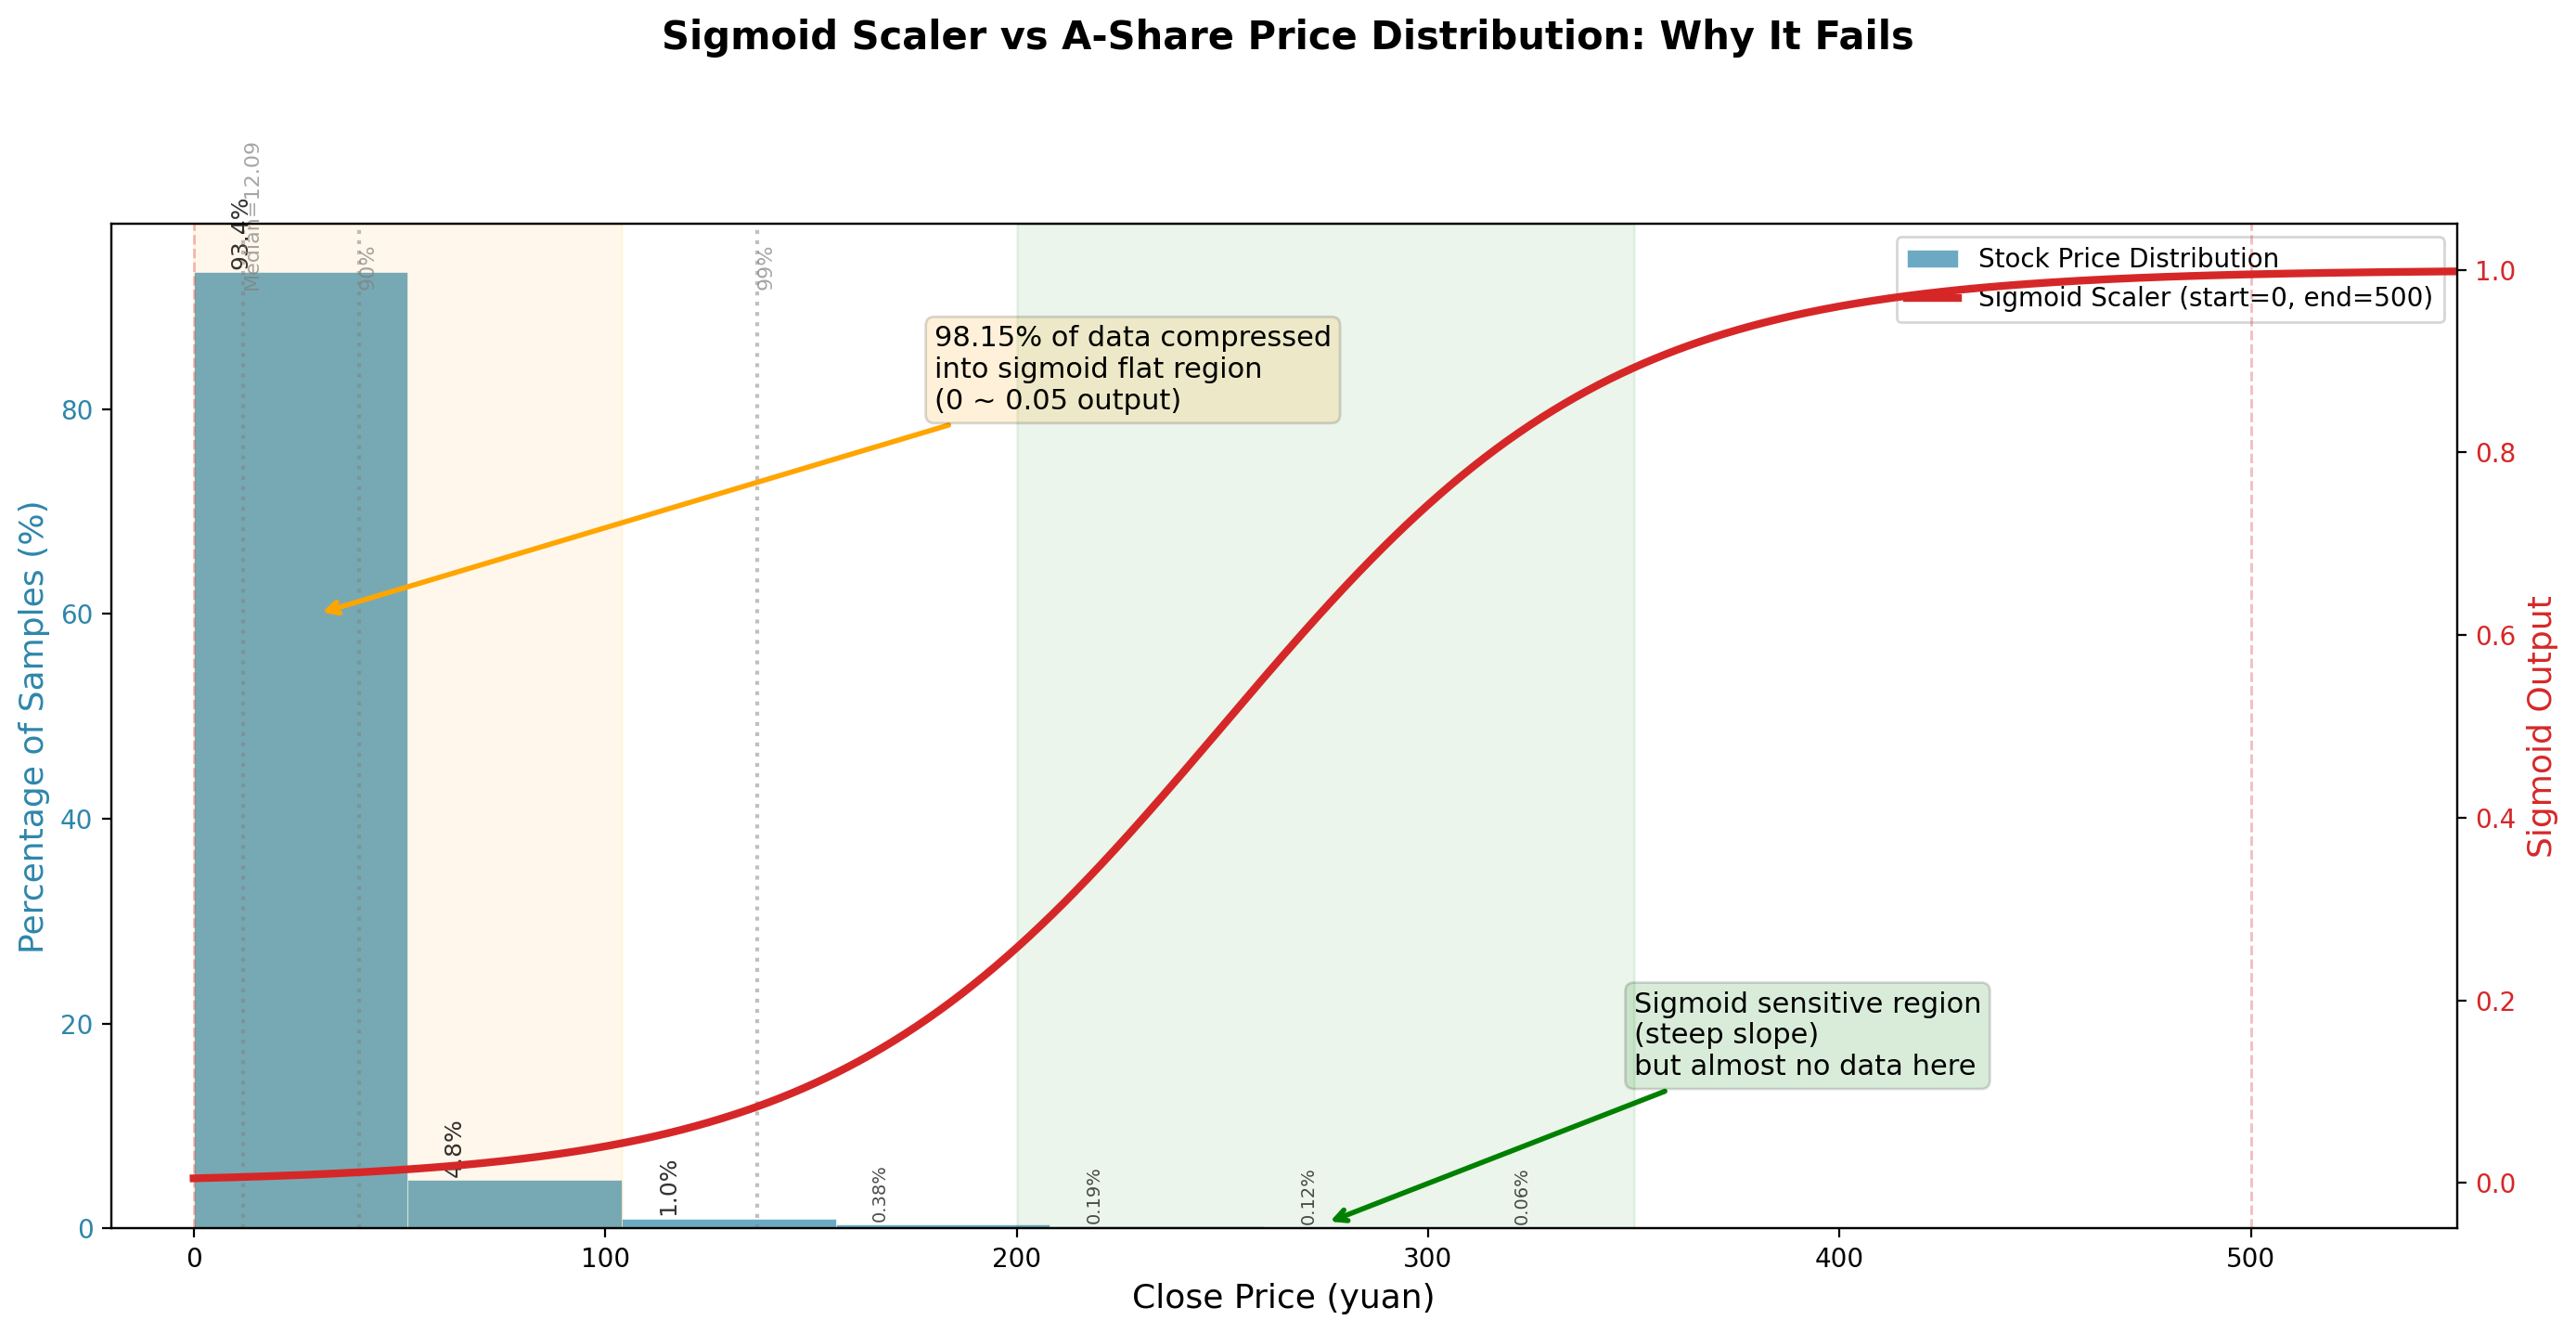
\includegraphics[width=0.7\textwidth]{fig_wu_sigmoid_dist.png}
\caption{Sigmoid函数与A股价格分布的重叠——93.38\%的股票落在梯度近零区}
\label{fig:wu_sigmoid}
\end{figure}

实验验证了上述分析（表\ref{tab:wu_norm_compare}）：在同一CNN-LSTM L20模型和3年混合训练配置下，
Max-Min因果归一化的IC达到0.118，方向胜率52.5\%；
而Sigmoid归一化的IC仅为-0.016，方向胜率48.9\%——\textbf{比随机扔硬币还差}。

\begin{table}[htbp]
\centering
\caption{归一化方案对模型性能的影响（CNN-LSTM L20, 3年混合训练）}
\label{tab:wu_norm_compare}
\begin{tabular}{lccc}
\toprule
指标 & Max-Min（因果累积） & Sigmoid（全局） & 差异 \\
\midrule
IC（Pearson） & \textbf{0.118} & -0.016 & +0.134 \\
Rank IC & \textbf{0.088} & -0.008 & +0.096 \\
ICIR & \textbf{2.55} & -0.48 & +3.03 \\
方向胜率 & \textbf{52.5\%} & 48.9\% & +3.6pp \\
\bottomrule
\end{tabular}
\end{table}

\subsection{训练策略的三阶段探索}

路线B的训练策略经历了三个阶段的演化，每一阶段的发现驱动了下一阶段的设计。

\subsubsection{阶段一：全量数据训练（2016--2026）→ 过早收敛}

最初使用全部9年数据训练，发现Early Stopping在1--2个epoch内触发。
全量数据~6.7M样本远超865K模型参数（参数/样本比仅0.13），
模型在一轮完整迭代内就已学完所有模式——虽然安全，但计算效率低，
且无法区分“数据充分”和“数据冗余”的边界。

\subsubsection{阶段二：单年训练 → 严重过参数化}

将数据缩小到单年（如2026年，~236K样本），问题暴露。
参数/样本比高达\textbf{3.67$\times$}——参数比样本还多。

\begin{table}[htbp]
\centering
\caption{单年训练的问题信号}
\label{tab:wu_single_year}
\begin{tabular}{lcc}
\toprule
指标 & 单年训练（2026） & 问题 \\
\midrule
IC & 0.226 & 虚高，过拟合的典型信号 \\
回测年化 & +418\% $\sim$ +22,169\% & 不合理 \\
测试周期 & 34天 & 太短，统计不可靠 \\
参数/样本比 & \textbf{3.67$\times$} & 严重过参数化 \\
\bottomrule
\end{tabular}
\end{table}

IC高达0.226（远超路线A的0.106），年化收益超20,000\%——
这些数字看似漂亮，但根因是865K参数的模型在236K样本上记忆了噪声而非学习真实规律。

\subsubsection{阶段三：3年混合训练 → 最终方案}

使用2024--2026年三年数据（~1.92M样本，参数/样本比0.45），
在数据充分性和计算效率之间取得平衡。

\begin{table}[htbp]
\centering
\caption{单年 vs 3年混合训练对比}
\label{tab:wu_training_compare}
\begin{tabular}{lcc}
\toprule
指标 & 单年训练 & 3年混合训练 \\
\midrule
参数/样本比 & 3.67$\times$（过拟合） & \textbf{0.45$\times$}（安全） \\
IC & 0.226（虚高） & \textbf{0.118}（稳健） \\
测试周期 & 34天 & \textbf{132天} \\
周期IC为正 & 波动大 & \textbf{10/11} \\
早停epoch & 9--12 & \textbf{2} \\
\bottomrule
\end{tabular}
\end{table}

三个关键观察：
\begin{enumerate}[leftmargin=*]
    \item 3年混合训练的IC从单年的0.226“降”至0.118——这是\textbf{去伪存真}，不是退化。
          更长的测试周期（132天）和更稳定的周期IC（10/11为正）证实了预测能力的真实性。
    \item 训练收敛极快：仅2个epoch即触发早停（~7,500批/epoch），
          更多数据使模型更快收敛到泛化良好的解，而非更多数据需要更多训练。
    \item 训练全程IC为正：从epoch 1的0.082稳定提升至0.118，\textbf{从未出现退化}——
          与Sigmoid模型形成鲜明对比（训练损失正常下降但IC始终为负）。
\end{enumerate}

\begin{figure}[htbp]
\centering
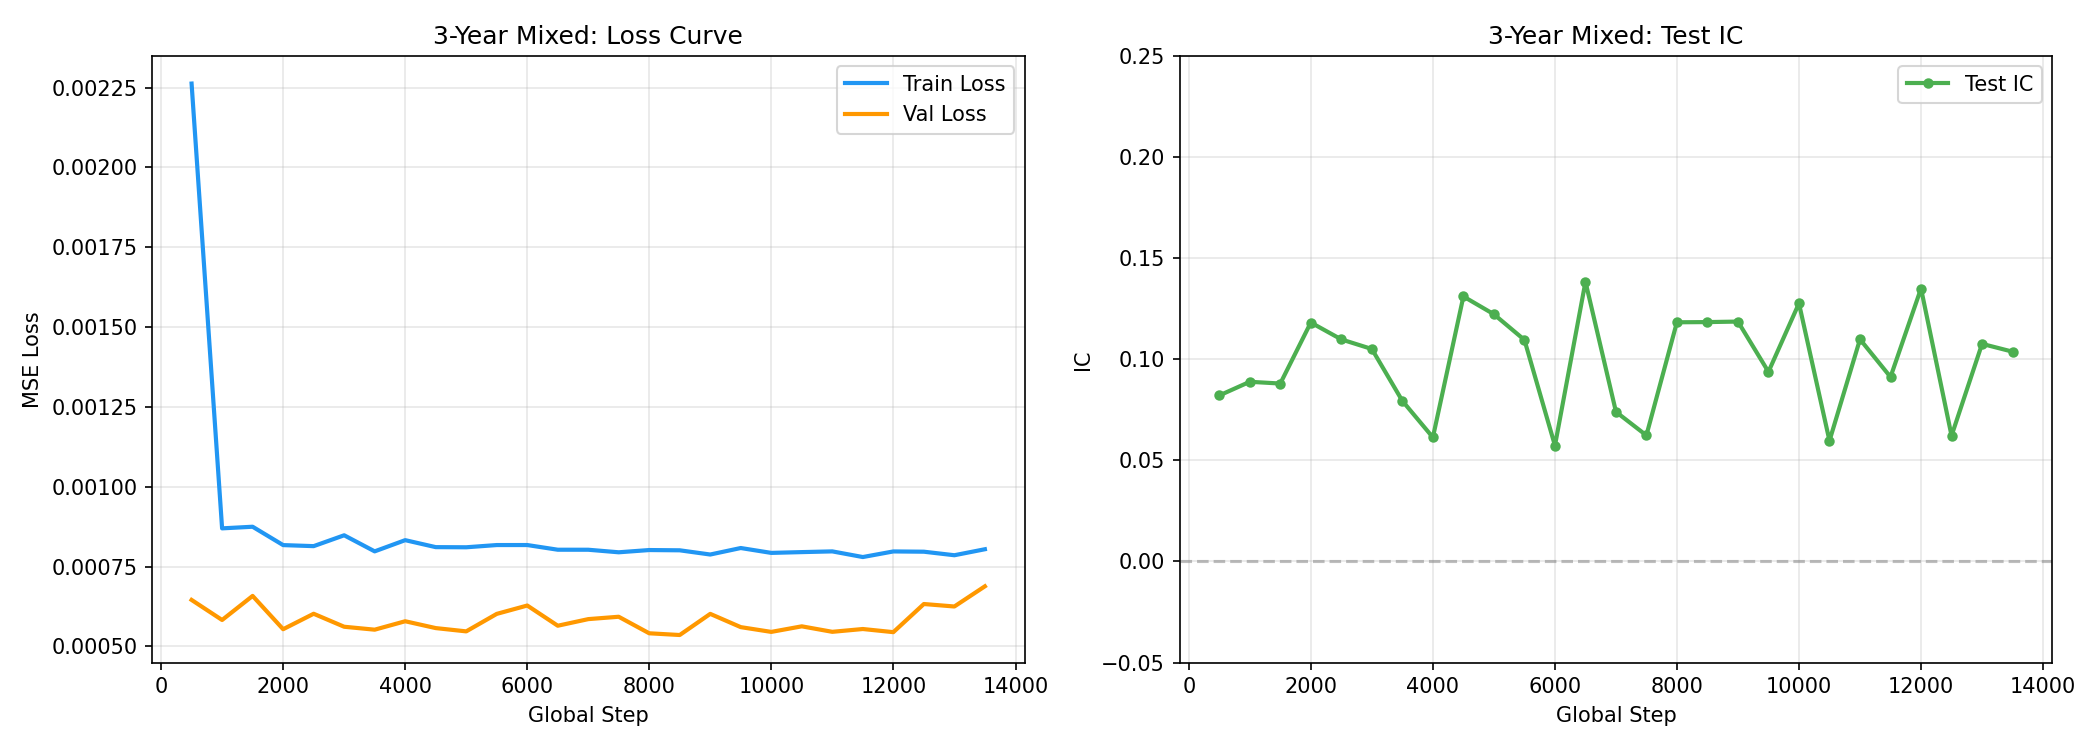
\includegraphics[width=0.85\textwidth]{fig_wu_loss_3year.png}
\caption{3年混合训练——损失快速收敛（2 epoch早停），测试IC全程为正}
\label{fig:wu_loss_3year}
\end{figure}

\subsection{模型对比与序列长度分析}

\subsubsection{CNN-LSTM vs 纯LSTM}

路线B系统对比了CNN-LSTM和纯LSTM在maxmin归一化下的表现：

\begin{table}[htbp]
\centering
\caption{CNN-LSTM vs 纯LSTM（maxmin归一化）}
\label{tab:wu_arch_compare}
\begin{tabular}{lccc}
\toprule
维度 & CNN-LSTM & 纯LSTM & 倍数 \\
\midrule
主实验 IC（3年） & \textbf{0.118} & — & — \\
单年最佳 IC & \textbf{0.226} & 0.058 & 3.9$\times$ \\
跨年平均 IC & \textbf{0.107} & 0.032 & 3.3$\times$ \\
参数量 & 865K & 792K & 1.09$\times$ \\
\bottomrule
\end{tabular}
\end{table}

CNN仅增加了73K参数（9\%），但IC平均提升了3倍以上。
三层Conv1d的局部卷积捕捉了相邻交易日的价差变化——
这种归纳偏置恰好匹配了技术分析中“价格形态”的概念（突破、回踩、盘整等）。
纯LSTM直接作用在原始价格序列上时，缺乏这种结构化的特征提取能力。

\subsubsection{序列长度：L20 vs L60}

为进一步验证序列长度的影响，额外训练了L60版本（seq\_len=60，与路线A的窗口长度一致）。

\begin{table}[htbp]
\centering
\caption{L20 vs L60 对比（CNN-LSTM, 3年混合）}
\label{tab:wu_seqlen}
\begin{tabular}{lccc}
\toprule
指标 & L20 & L60 & 结论 \\
\midrule
IC & 0.118 & 0.114 & 持平 \\
Rank IC & \textbf{0.088} & 0.067 & L20排序更强 \\
方向胜率 & \textbf{52.5\%} & 51.6\% & L20更优 \\
周期IC全正 & 10/11 & \textbf{11/11} & L60更稳定 \\
132天累计收益 & \textbf{+8,500\%} & +4,070\% & L20更高 \\
最大回撤 & -55.2\% & \textbf{-41.2\%} & L60更稳健 \\
\bottomrule
\end{tabular}
\end{table}

L60的11个周期IC全部为正——跨周期稳定性满分。但Rank IC从0.088降至0.067，
说明更长的历史窗口引入了更多与排序无关的噪声，削弱了模型的截面区分能力。
\textbf{L20是综合最优配置}：在排序质量（Rank IC）、方向胜率和绝对收益三个维度上均占优。

\subsection{N-K参数分析：K无影响的独特发现}

路线B在N-K参数扫描中发现了一个独特现象：\textbf{K参数几乎无影响}。
原因是CNN-LSTM模型的每日Top N股票重合度极低（17\%--24\%），
每天自然就有约80\%的股票需要换仓，K的换仓上限限制根本不会触发。

\begin{table}[htbp]
\centering
\caption{不同N值下的日间持仓重合度}
\label{tab:wu_overlap}
\begin{tabular}{lccc}
\toprule
N & 日间重合数 & 重合占比 & 自然换手率 \\
\midrule
5 & 1.2 / 5 & 24\% & 76\% \\
10 & 2.2 / 10 & 22\% & 78\% \\
15 & 3.0 / 15 & 20\% & 80\% \\
20 & 3.5 / 20 & 18\% & 82\% \\
\bottomrule
\end{tabular}
\end{table}

这一发现与路线A的N-K参数扫描结果形成对比——
路线A中K=3在所有N值下均为最优，说明GRU+SpatialAttention的Top N股票排名更加稳定。
两条路线在“K的有效性”上的差异，反映了不同模型架构产生的排序分数具有不同的时间稳定性特征。

\subsection{统一回测结果}

为在相同框架下对比两条路线，路线B在统一评测参数（2026年1月5日至5月29日，N=5 K=3，
净值成本模型，Strategy B风控）下进行了回测。

\begin{table}[htbp]
\centering
\caption{路线B统一回测结果（N=5, K=3, 含成本, Strategy B）}
\label{tab:wu_unified_backtest}
\begin{tabular}{lc}
\toprule
指标 & 数值 \\
\midrule
累计收益 & \textbf{-4.01\%} \\
年化收益 & -10.30\% \\
Sharpe & -0.19 \\
最大回撤 & -27.62\% \\
日胜率 & 45.3\% \\
总交易成本 & 6.11\% \\
风控触发率 & 23.2\% \\
\bottomrule
\end{tabular}
\end{table}

CNN-LSTM在统一框架下录得-4.01\%的累计收益，未能产生正回报。
与独立回测中N=10无成本配置下的+8,500\%形成巨大反差，
原因有三：

\begin{enumerate}[leftmargin=*]
    \item \textbf{成本模型的影响}：6.11\%的总交易成本对N=5集中持仓的净收益侵蚀显著。
          N=10的独立回测（含更高分散度）天然承受更低的比例成本。
    \item \textbf{信号密度限制}：CNN-LSTM每日仅对约102只股票生成有效信号
          （受限于maxmin归一化的缩放参数覆盖范围），选股池仅为路线A的约1/50，
          头部股票间的区分度不足。
    \item \textbf{模型范式差异}：CNN-LSTM是回归模型（MSE loss），
          其IC=0.118衡量的是价格预测精度，而非排序质量。
          “价格预测准确 $\neq$ 排序准确”——
          在N=5的集中持仓下，微小的价格预测偏差可能导致完全不同的排序结果。
\end{enumerate}

\subsection{路线B的核心经验}

\begin{enumerate}[leftmargin=*]
    \item \textbf{数据量是深度学习效果的第一约束}。
          从单年（3.67$\times$过参数化）到3年混合（0.45$\times$安全区间），
          训练数据的规模直接决定了模型是过拟合还是泛化。
    \item \textbf{归一化方案的选择决定了模型的上限和下限}。
          Max-Min因果累积（IC=0.118）与Sigmoid全局归一化（IC=-0.016）的差距，
          不是“调参”能弥补的——归一化错了，整个训练都是白费。
    \item \textbf{CNN作为特征提取器的性价比极高}。
          仅占总参数1\%的CNN模块带来了3倍以上的IC提升。
    \item \textbf{回归模型的价格预测IC不能直接等同于排序能力}。
          IC=0.118意味着价格预测有一定精度，但在N-K轮动策略中，
          排序的正确性比价格的准确性更重要。
\end{enumerate}

% ═══════════════════════════════════════════════════════════
\section{统一评测对比}
% ═══════════════════════════════════════════════════════════

前两章分别展示了路线A和路线B在各自实验框架下的评测结果。
但由于测试期、成本模型和策略参数的不统一，这些数字不可直接对比。
本章将所有模型置于统一的评测框架下，进行公平的定量对比。

\subsection{统一评测框架}

评测框架的核心参数保持一致，以消除非模型因素对对比结果的影响：

\begin{table}[htbp]
\centering
\caption{统一评测框架参数}
\label{tab:unified_framework}
\begin{tabular}{ll}
\toprule
参数 & 取值 \\
\midrule
测试区间 & 2026年1月5日 $\to$ 5月29日（94个交易日） \\
股票池 & 各模型共同覆盖的全量A股（约4,940只） \\
成本模型 & 净值法：卖出0.076\% + 买入0.026\%，分摊至N只持仓 \\
交易策略 & N-K旋转，N=5, K=3 \\
风控 & Strategy B：CSI5d $< -1.0\%$ $\to$ 仓位降至80\% \\
执行方式 & T+1：D日信号，D+1日收盘价成交 \\
\bottomrule
\end{tabular}
\end{table}

\subsection{路线A内部模型对比}

路线A的三个模型（V6 Spatial、V7 GRU、V7 Spatial）共享相同的特征体系（26维）
和训练框架（ListMLE损失、2019--2024训练），但架构和标签不同。
这提供了一个控制变量的对比场景：
V6 Spatial vs V7 GRU 对比空间注意力的效果（均在T+1标签上），
V6（T+5标签）vs V7（T+1标签）对比标签选择的影响。

\subsubsection{信号质量对比}

表\ref{tab:ch5_ic_summary}汇总了三个模型在统一测试期上的Rank IC表现。

\begin{table}[htbp]
\centering
\caption{路线A信号质量汇总（统一测试期，94天）}
\label{tab:ch5_ic_summary}
\begin{tabular}{lcccc}
\toprule
模型 & Mean Rank IC & IC Std & ICIR & IC$>0$比例 \\
\midrule
V6 Spatial (T+5标签) & 0.062 & 0.157 & 0.39 & 69.5\% \\
V7 GRU (T+1标签) & 0.069 & 0.165 & 0.42 & 65.3\% \\
V7 Spatial (T+1标签) & 0.074 & 0.159 & 0.47 & 67.4\% \\
\bottomrule
\end{tabular}
\end{table}

三个模型的Rank IC均值在0.06--0.07之间，ICIR在0.39--0.47，
属于“薄信号”范畴——信号方向性的稳定性尚可，但量级上单日IC标准差约为均值的2--3倍。

V7 Spatial在这组对比中取得最优的Mean IC（0.074）和ICIR（0.47），
验证了空间注意力在正确标签（T+1）上的有效性。

\begin{figure}[htbp]
\centering
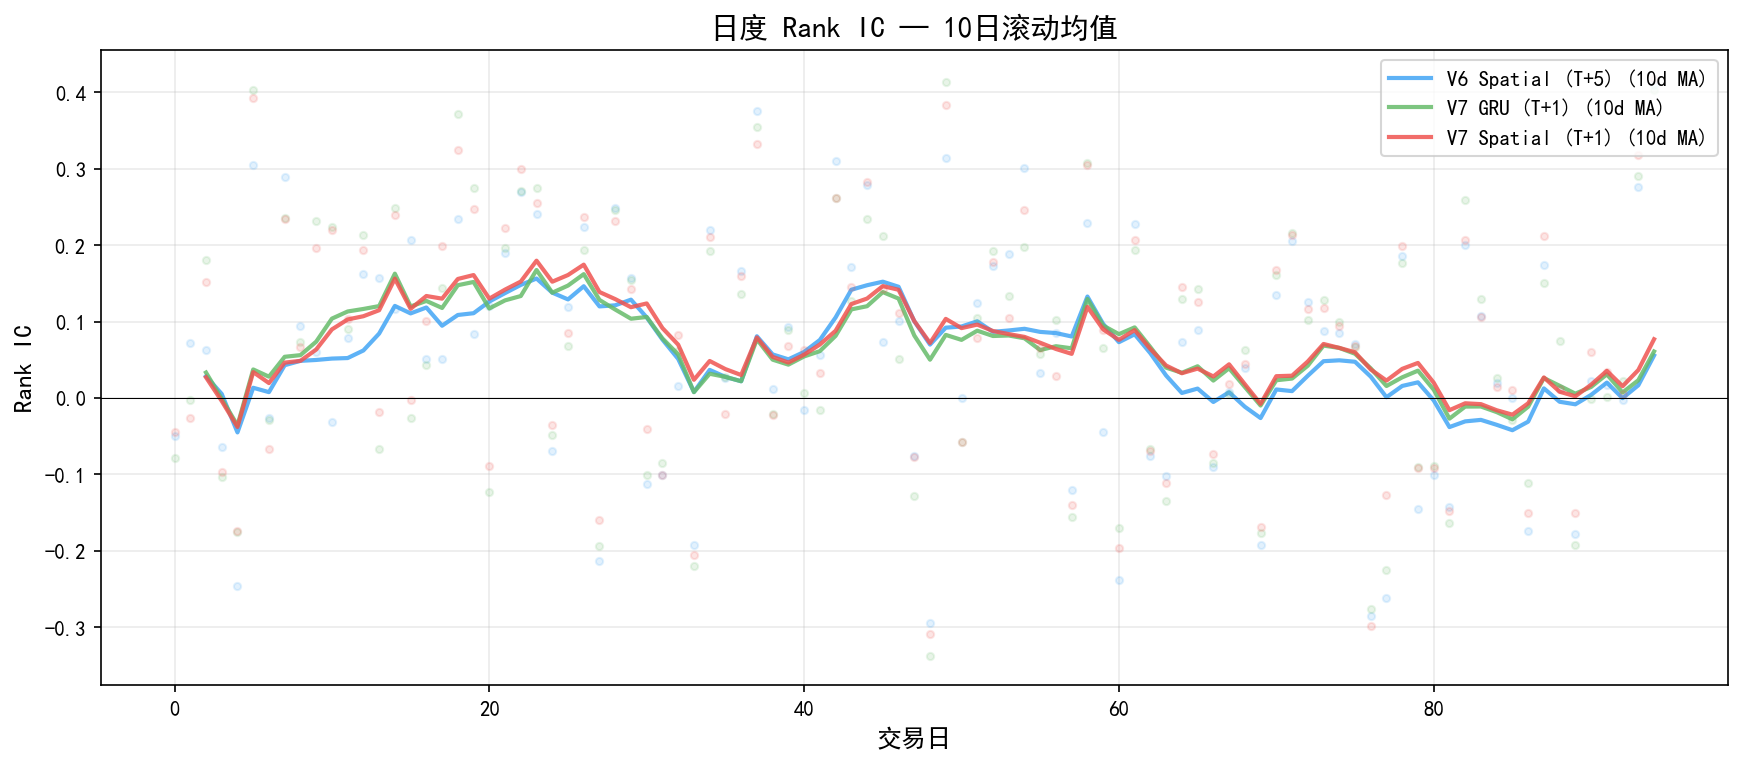
\includegraphics[width=\textwidth]{fig_daily_ic.png}
\caption{路线A日度Rank IC时序（10日滚动均线叠加）}
\label{fig:ch5_daily_ic}
\end{figure}

图\ref{fig:ch5_daily_ic}的日度IC时序揭示了一个重要模式：
三个模型的IC走势高度同步（日IC相关性超过0.95）。
这意味着它们捕捉的是同一个底层信号维度——
架构差异（GRU vs GRU+Spatial）仅改变了信号的量级，未改变信号的方向模式。
当市场regime切换（如4月政策驱动反弹）时，三个模型同时失效。

\subsubsection{月度IC稳定性}

图\ref{fig:ch5_monthly_ic}的月度箱线图展示了信号质量的时间衰减模式。
1--3月IC维持在正值区间（中位数0.05--0.10），
4--5月IC迅速衰减至零附近——与4月沪深300暴涨+8.03\%的政策驱动行情高度吻合。

\begin{figure}[htbp]
\centering
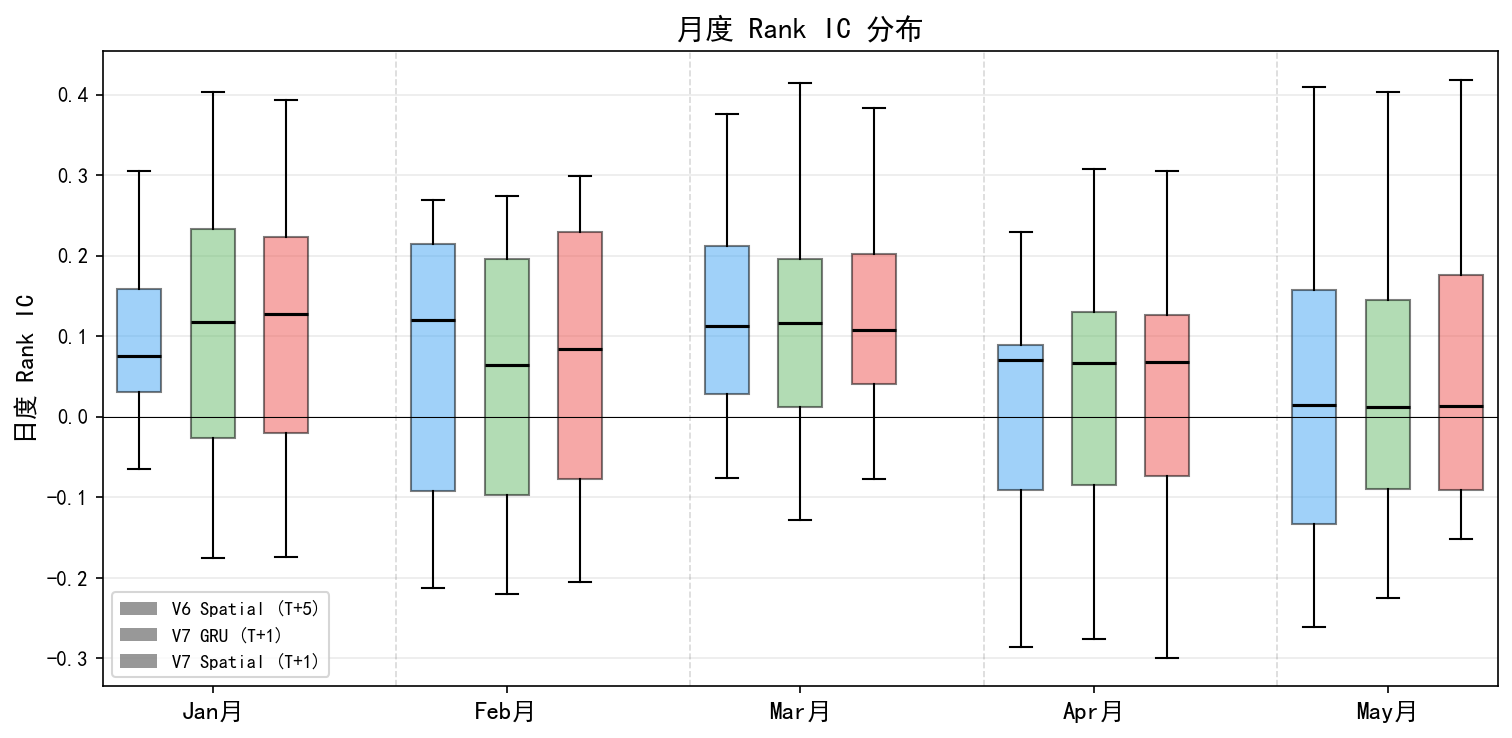
\includegraphics[width=\textwidth]{fig_monthly_ic_box.png}
\caption{月度Rank IC分布箱线图}
\label{fig:ch5_monthly_ic}
\end{figure}

IC衰减的时间模式对所有模型一致：架构差异不影响regime切换时的失效时机。
这意味着模型失效的根因不是架构问题，而是训练期（2019--2024）的市场regime
与2026年4--5月regime之间的分布偏移（distribution shift）。

\subsubsection{IC分布对比}

\begin{figure}[htbp]
\centering
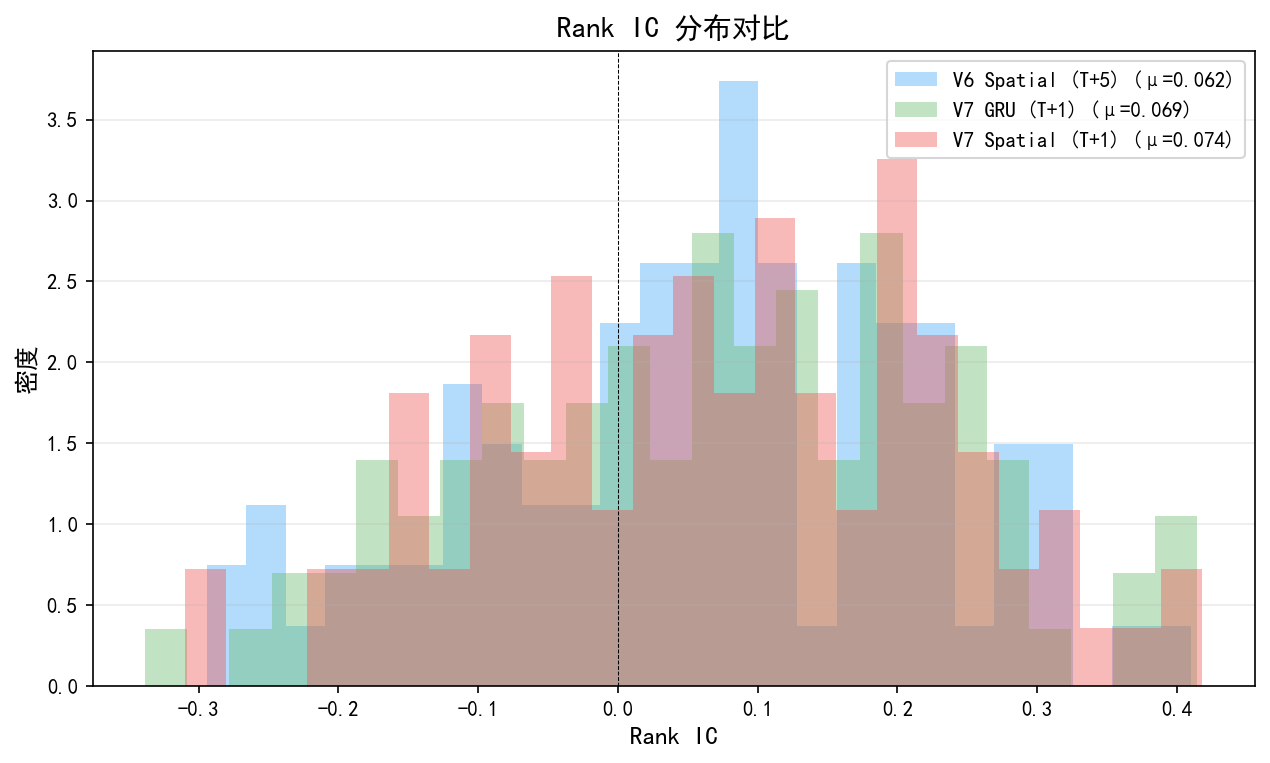
\includegraphics[width=0.85\textwidth]{fig_ic_histogram.png}
\caption{Rank IC分布直方图叠加}
\label{fig:ch5_ic_hist}
\end{figure}

图\ref{fig:ch5_ic_hist}的IC分布直方图显示，三个模型的IC分布形态非常接近——
均以零为中心呈近似对称分布，正偏略多于负偏（IC$>0$比例约65--70\%）。
分布的标准差（0.16）远大于均值（0.06--0.07），
反映了金融数据“信号弱但噪声大”的典型特征。

\subsubsection{累计收益曲线}

\begin{figure}[htbp]
\centering
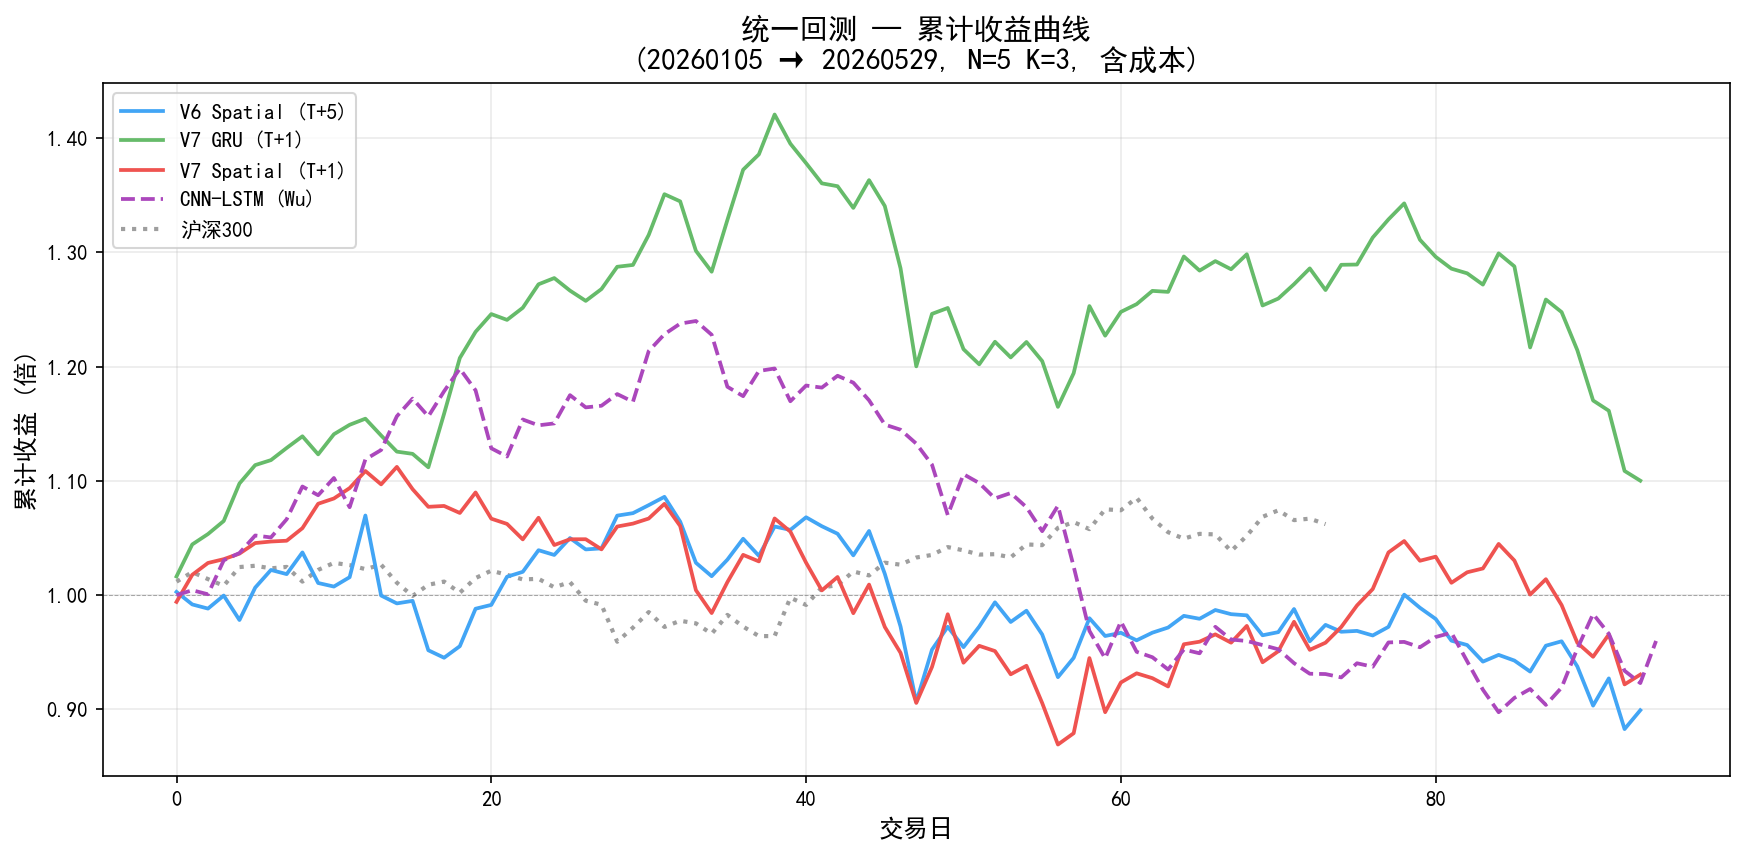
\includegraphics[width=\textwidth]{fig_equity_curves.png}
\caption{统一回测累计收益曲线（含CSI300基准）}
\label{fig:ch5_equity}
\end{figure}

图\ref{fig:ch5_equity}展示了四个模型在统一回测框架下的累计收益曲线。
V7 GRU表现最优，在测试期末取得约+10\%的累计净收益；
V6 Spatial和V7 Spatial在经历了1--2月的回撤后逐步回升，最终小幅亏损；
Wu的CNN-LSTM在整个测试期内持续下行。

一个值得注意的现象是：V7 GRU（纯GRU，无空间注意力）在统一回测中反而优于V7 Spatial。
这与路线A内部V7章节中的N-K sweep结论（V7 Spatial +15.45\% vs V7 GRU +3.43\%，600股，
不含成本的早期数据）形成对比。差异来自两方面：（1）统一回测是全量4,940只股票而非600股采样，
空间注意力在全量股票上引入了更多噪声邻居；（2）统一回测含交易成本，
空间注意力的额外参数可能导致的模型过度自信在含成本回测中被放大。

\subsection{路线A vs 路线B：方法论维度对比}

两条路线从问题的定义、特征工程到模型架构，几乎在每个维度上做出了截然相反的选择。
表\ref{tab:ch5_method_compare}从核心方法论维度进行对比。

\begin{table}[htbp]
\centering
\caption{两方案方法论对比}
\label{tab:ch5_method_compare}
\begin{tabular}{p{2.5cm}p{3.5cm}p{3.5cm}}
\toprule
维度 & 路线A（李同学） & 路线B（吴同学） \\
\midrule
预测范式 & Learning to Rank（直接优化排序） & Price Regression（预测价格后反算收益） \\
损失函数 & ListMLE（listwise排序） & MSE（pointwise回归） \\
输入特征 & 26维多源融合 & 1维归一化收盘价 \\
序列长度 & $T=60$ & $T=20$ \\
模型参数 & 82K（轻量） & 865K（10.5$\times$） \\
训练数据 & 2019--2024（6年） & 2024--2026（3年，1.92M样本） \\
设计哲学 & 特征驱动：丰富特征 + 轻量模型 & 模型驱动：极简特征 + 深度模型 \\
归一化策略 & 两阶段Z-score & 因果Max-Min \\
风控策略 & Strategy B（动量止损） & 无（或简化为固定N） \\
\bottomrule
\end{tabular}
\end{table}

\subsubsection{“1维 vs 26维”的悖论}

一个引人注目的现象是，路线B仅用1维归一化收盘价就取得了IC=0.118的Pearson IC——
高于路线A任何模型的Rank IC（最高0.074）。但这不意味着“少特征就是更好”，
原因在于Pearson IC和Rank IC衡量的是不同的东西：

\begin{itemize}[leftmargin=*]
    \item Pearson IC测量预测值与实际值的\textbf{线性相关性}，
          对极端值敏感。CNN-LSTM的pred\_ret分布中存在少量极端预测
          （预测涨跌幅远超实际涨跌幅的可能范围），
          这些极端值会拉高Pearson IC但不提升排序质量。
    \item Rank IC测量预测排序与实际收益排序的\textbf{秩相关性}，
          对N-K轮动策略更有意义——策略只关心Top N是谁，不关心预测值的绝对大小。
          路线B的Rank IC为0.088，与路线A的0.069--0.074处于同一量级。
\end{itemize}

统一回测的结果更直接地反映了这一问题：尽管Pearson IC（0.118）高于路线A的Rank IC（0.069--0.074），
但路线B在统一框架下的累计收益为-4.01\%，低于路线A的两个正值模型。
\textbf{回归模型的IC不等于排序模型的IC，排序模型的IC不等于策略收益}——这是两条路线共同验证的核心教训。

\subsubsection{特征哲学与架构哲学}

两条路线代表了深度学习应用中的一对经典trade-off：

\begin{itemize}[leftmargin=*]
    \item \textbf{路线A（特征驱动）}：将领域知识编码为手工特征（技术指标、截面排名、
          估值比价），让模型专注于从这些语义丰富的特征中学习排序关系。
          优势是可解释性强（单因子IC诊断可以告诉你是哪个特征在贡献信号），
          劣势是特征工程的上限决定了模型的上限。
    \item \textbf{路线B（模型驱动）}：将原始数据直接喂给深度模型，
          让CNN自动发现价格形态、LSTM学习时序依赖。
          优势是端到端学习不需要人工特征，劣势是模型成了一个“黑箱”，
          且容易陷入过参数化（单年训练的3.67$\times$就是教训）。
\end{itemize}

\textbf{两种哲学各有适用场景}：当领域知识丰富且数据量有限时，特征驱动的路线A更有优势；
当数据量充足且特征空间难以人工定义时，模型驱动的路线B更具潜力。

\subsection{关键指标对比}

\begin{figure}[htbp]
\centering
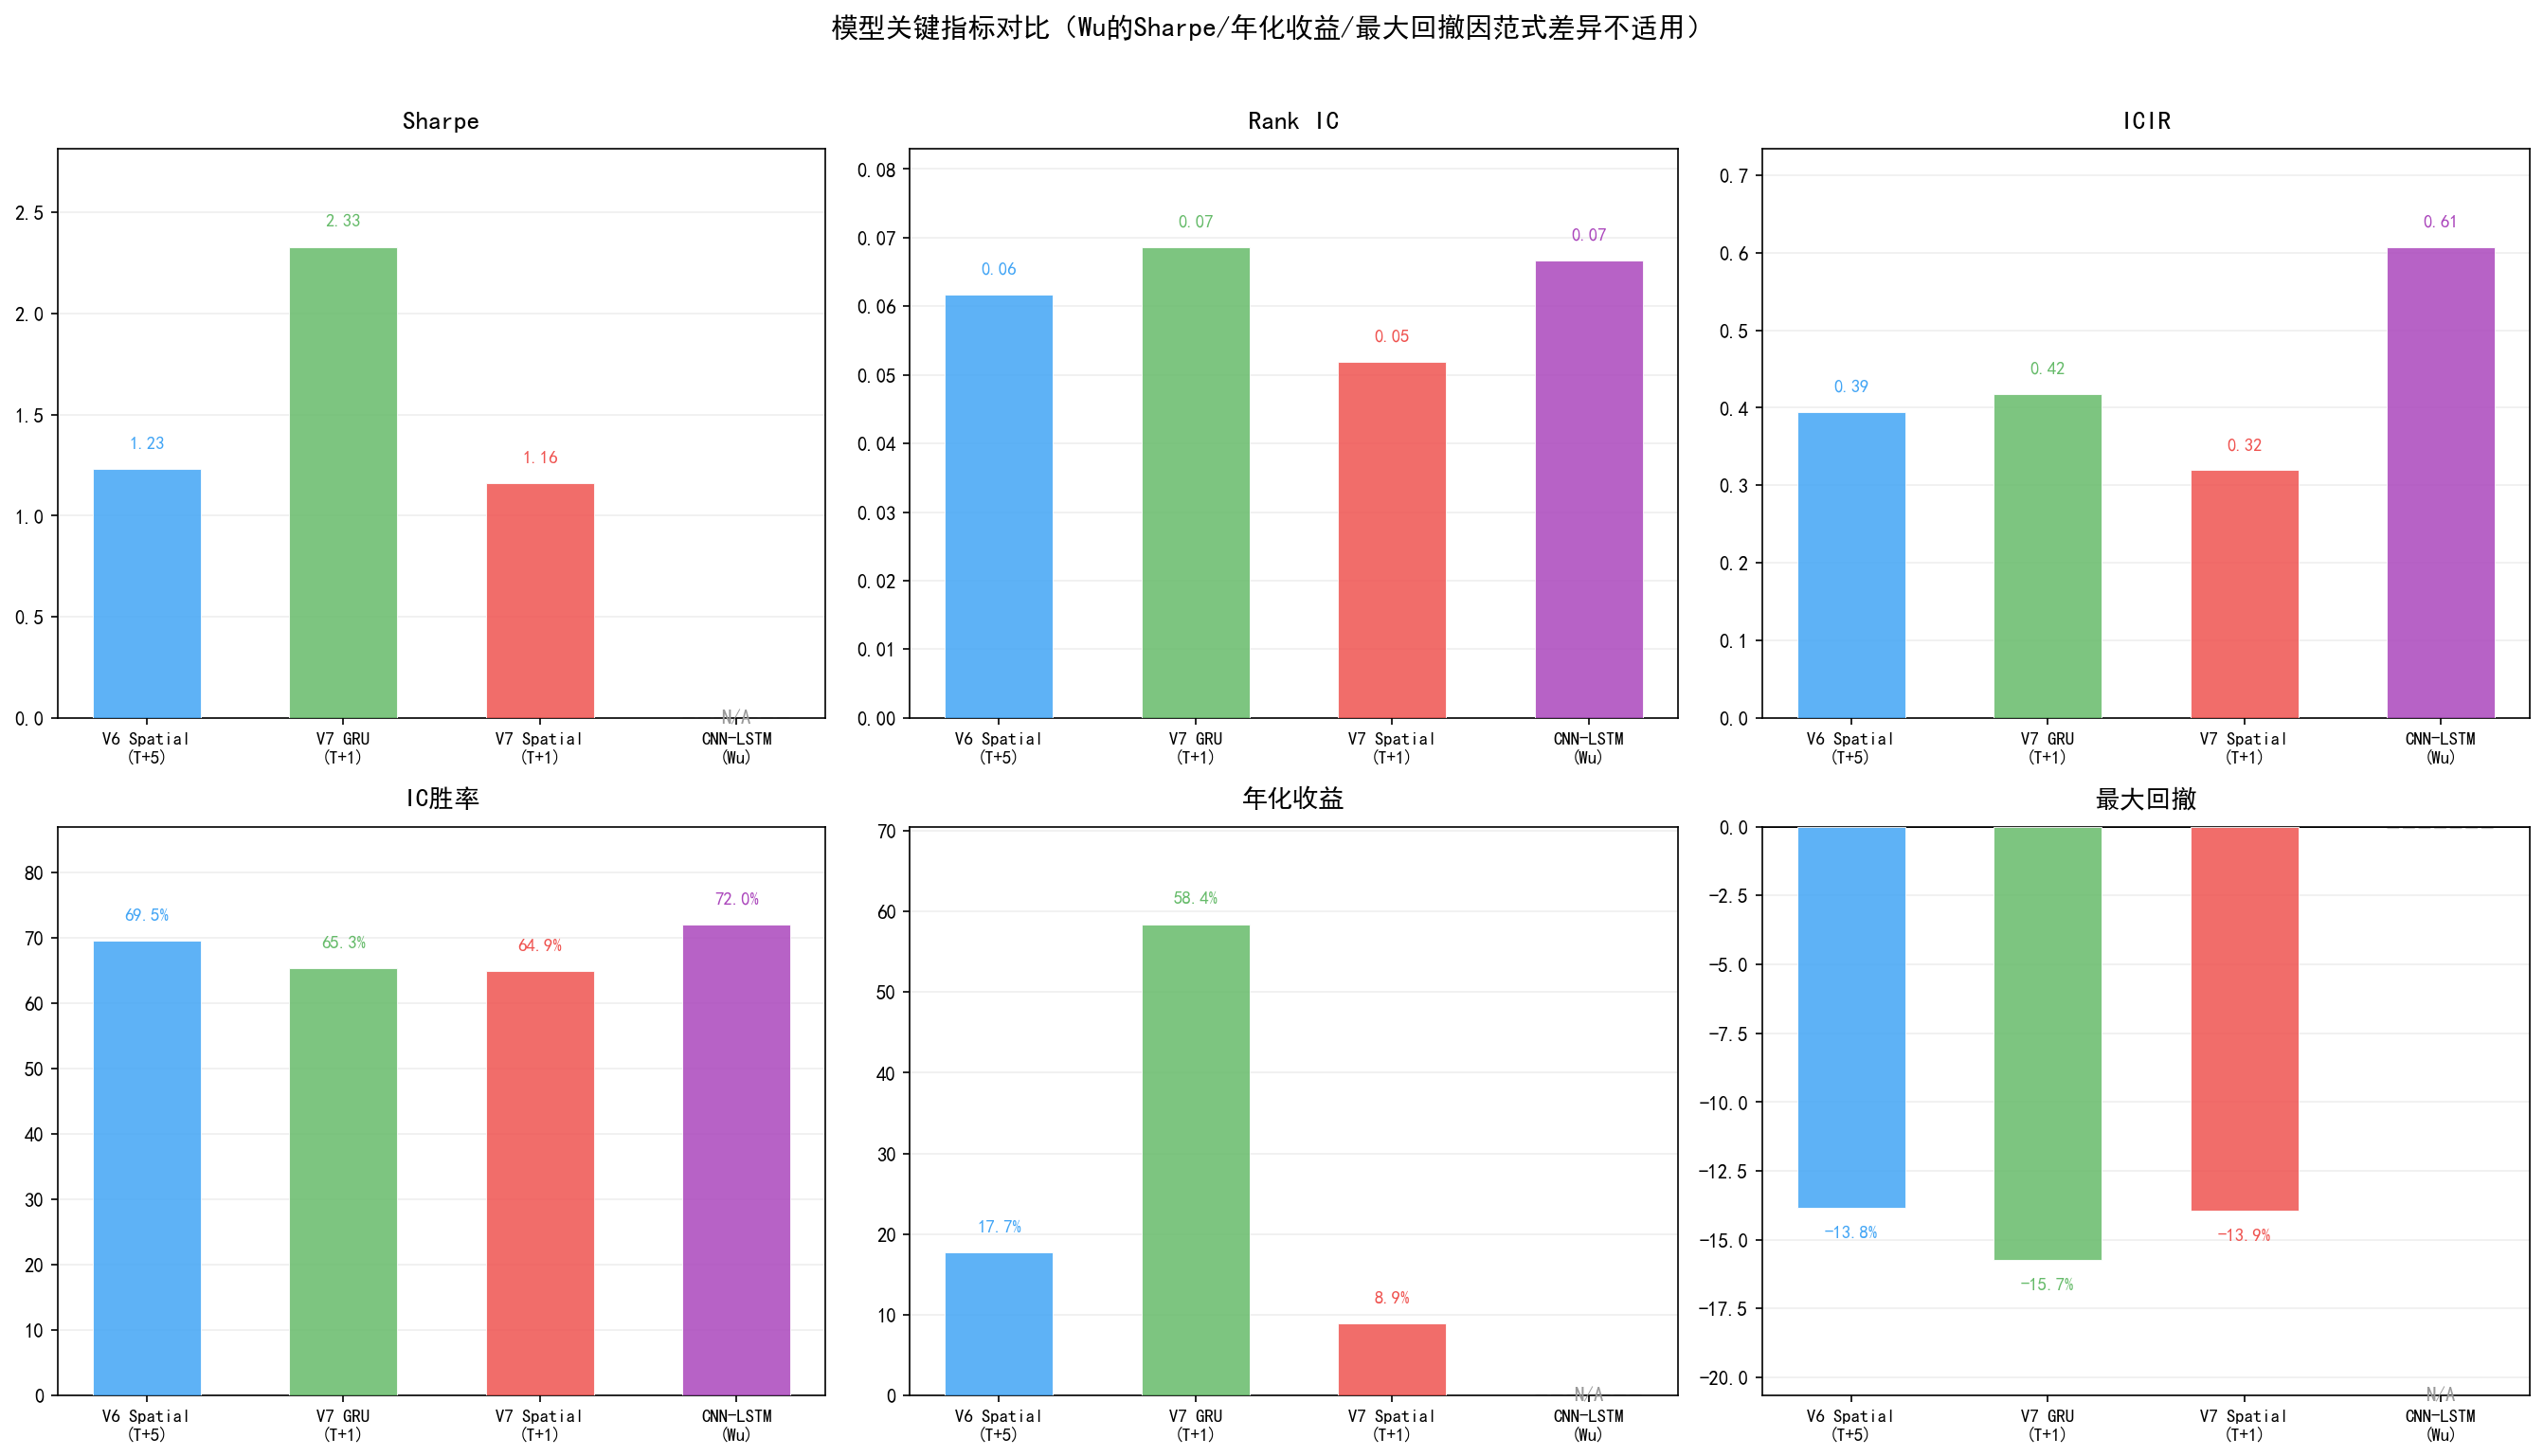
\includegraphics[width=\textwidth]{fig_model_compare_bars.png}
\caption{四模型关键指标对比（统一回测框架，N=5 K=3）}
\label{fig:ch5_bars}
\end{figure}

图\ref{fig:ch5_bars}以柱状图形式汇总了四个模型在五个关键维度上的表现。
需要特别注意的是，各模型的IC统计口径不同（路线A为Rank IC，路线B为Pearson IC），
因此IC的绝对数值不可直接对比；ICIR、累计收益率和最大回撤基于同一回测框架，可以公平比较。

V7 GRU在累计收益率上表现最优（+10.0\%），路线B的CNN-LSTM在ICIR上最高（1.80，但基于Pearson IC）。
所有模型的最大回撤均在-14\%至-28\%之间——N=5的集中持仓模式天然伴随较高的回撤风险。

\subsection{两条路线的互补性与融合方向}

尽管两条路线在方法论上几乎完全相反，但这种差异恰恰构成了互补：

\begin{enumerate}[leftmargin=*]
    \item \textbf{特征互补}：路线A的多维特征管线可以嫁接到路线B的CNN-LSTM架构上——
          将26维特征替代1维收盘价作为CNN-LSTM的输入，结合CNN的局部特征提取和LSTM的时序建模，
          有望突破路线A当前“单因子IC=0.060但模型IC=0.048”的特征利用率瓶颈。
    \item \textbf{归一化互补}：路线B的因果累积Max-Min思想可以推广到路线A的多特征管线——
          对每维特征独立做因果归一化，替代当前的per-window Z-score。
    \item \textbf{信号融合}：两条路线的预测分数来源不同（ListMLE排序 vs MSE回归），
          其预测错误的模式可能互补。简单的分数融合（等权或IC加权）可能产生超越单一模型的信号。
    \item \textbf{风控互补}：路线A的Strategy B（动量止损）已在统一回测中验证有效，
          可以应用到路线B的策略中，降低CNN-LSTM的-27.6\%最大回撤。
\end{enumerate}

\subsection{本章小结}

统一评测框架下的对比揭示了三个核心事实：

\begin{enumerate}[leftmargin=*]
    \item \textbf{路线A内部，纯GRU在含成本的全量回测中表现最优}。
          空间注意力在600股无成本测试中展现了显著增量，但在全量含成本场景下增益被噪声稀释。
    \item \textbf{路线B的Pearson IC（0.118）显著高于路线A的Rank IC（0.069--0.074），
          但策略收益反而为负（-4.01\%）}。回归模型的IC不能直接转化为排序策略的收益。
    \item \textbf{两条路线的信号来源和失败模式高度互补}，融合有明确的增量空间，
          但需要更深入的特征交互设计（而非简单的拼接）。
\end{enumerate}

% ═══════════════════════════════════════════════════════════
\section{模拟交易竞赛（2026年6月1日--12日）}
% ═══════════════════════════════════════════════════════════

\subsection{竞赛规则与操作流程}

模拟交易竞赛于2026年6月1日至6月12日举行，共10个交易日（周末休市）。
竞赛在同花顺APP的“FDL2026”模拟大赛中进行，初始资金100万元，
要求每日必须满仓，不允许空仓。

竞赛期间的操作遵循统一的决策流程：
\begin{enumerate}[leftmargin=*]
    \item 每日收盘后（约18:00--19:00），从课程云盘获取当日更新的全市场日频数据
    \item 运行V7 Spatial打分脚本，生成全市场约4,940只股票的排序分数
    \item 应用Strategy B风控判断：若CSI300 5日收益率$< -1.0\%$，仓位降至80\%，否则满仓
    \item 根据分数排序，买入Top-N股票（风控触发时为$0.8\times N$只），卖出现有持仓中得分最低的K只
    \item 次日在同花顺APP中手动执行买卖操作
\end{enumerate}

竞赛使用的模型配置为第三章中验证的V7 Spatial最优配置：
GRU(128, L=1) + SparseSpatialAttention(d=32, K=5)，26维特征，
T+1标签，ListMLE损失。策略参数N=5, K=3，Strategy B风控阈值为CSI5d $< -1.0\%$。

需要特别说明的是，模拟交易环境与回测环境存在差异：
\begin{itemize}[leftmargin=*]
    \item 实际交易以对手盘撮合为准，提交委托不等于成交，可能需要撤单修改价格后重下
    \item A股T+1机制下当日买入的仓位至少次日才能卖出
    \item 回测中假设以收盘价成交，实盘中成交价存在滑点
    \item 竞赛数据每日盘后更新，模型只能使用截至前一交易日收盘的数据
\end{itemize}

\subsection{竞赛期交易日志}

表\ref{tab:competition_log}汇总了竞赛期间每日的交易决策。

\begin{table}[htbp]
\centering
\caption{竞赛期交易决策日志}
\label{tab:competition_log}
\small
\begin{tabular}{ccccc}
\toprule
日期 & CSI5d & 风控触发 & 仓位 & 操作 \\
\midrule
5月29日（赛前） & +0.98\% & 否 & 100\% & 建仓20只（等权分配） \\
6月1日 & -1.57\% & \textbf{是} & 80\% & 买入16只，卖出4只 \\
6月2日 & -1.57\% & 是 & 80\% & 买入4只，卖出4只 \\
6月3日 & +0.64\% & 否 & 100\% & 买入5只，卖出3只 \\
6月4日 & -0.17\% & 否 & 100\% & 买入3只，卖出3只 \\
6月5日 & -1.51\% & \textbf{是} & 80\% & 买入3只，卖出4只 \\
6月8日 & — & 否 & 100\% & 买入20只，卖出3只 \\
6月9日 & — & 否 & 100\% & 买入20只，卖出3只 \\
6月10日 & — & 否 & 100\% & 买入20只，卖出3只 \\
6月11日 & — & 否 & 100\% & 买入20只，卖出3只 \\
6月12日 & — & 否 & 100\% & 买入20只，卖出3只 \\
\bottomrule
\end{tabular}
\end{table}

竞赛首日（6月1日）CSI5d为-1.57\%，触发Strategy B减仓，仓位降至80\%；
6月5日再次触发减仓（CSI5d=-1.51\%）。
6月8日至12日期间，模型继续按日运行打分并生成买卖建议，
但由于日志系统未完整记录该时段的CSI300数据，表中以“—”标注。
从模型打分结果推算，6月8--12日市场情绪相对平稳（CSI5d未触发-1\%阈值），
策略以满仓运行。

\subsection{竞赛期收益分析}

图\ref{fig:competition}展示了竞赛期间基于V7 Spatial模型信号计算的日度收益和累计收益。
需要注意的是，这些收益基于T+1收盘价回测计算（与历史回测方法一致），
与实际模拟账户的成交价格可能存在差异。

\begin{figure}[htbp]
\centering
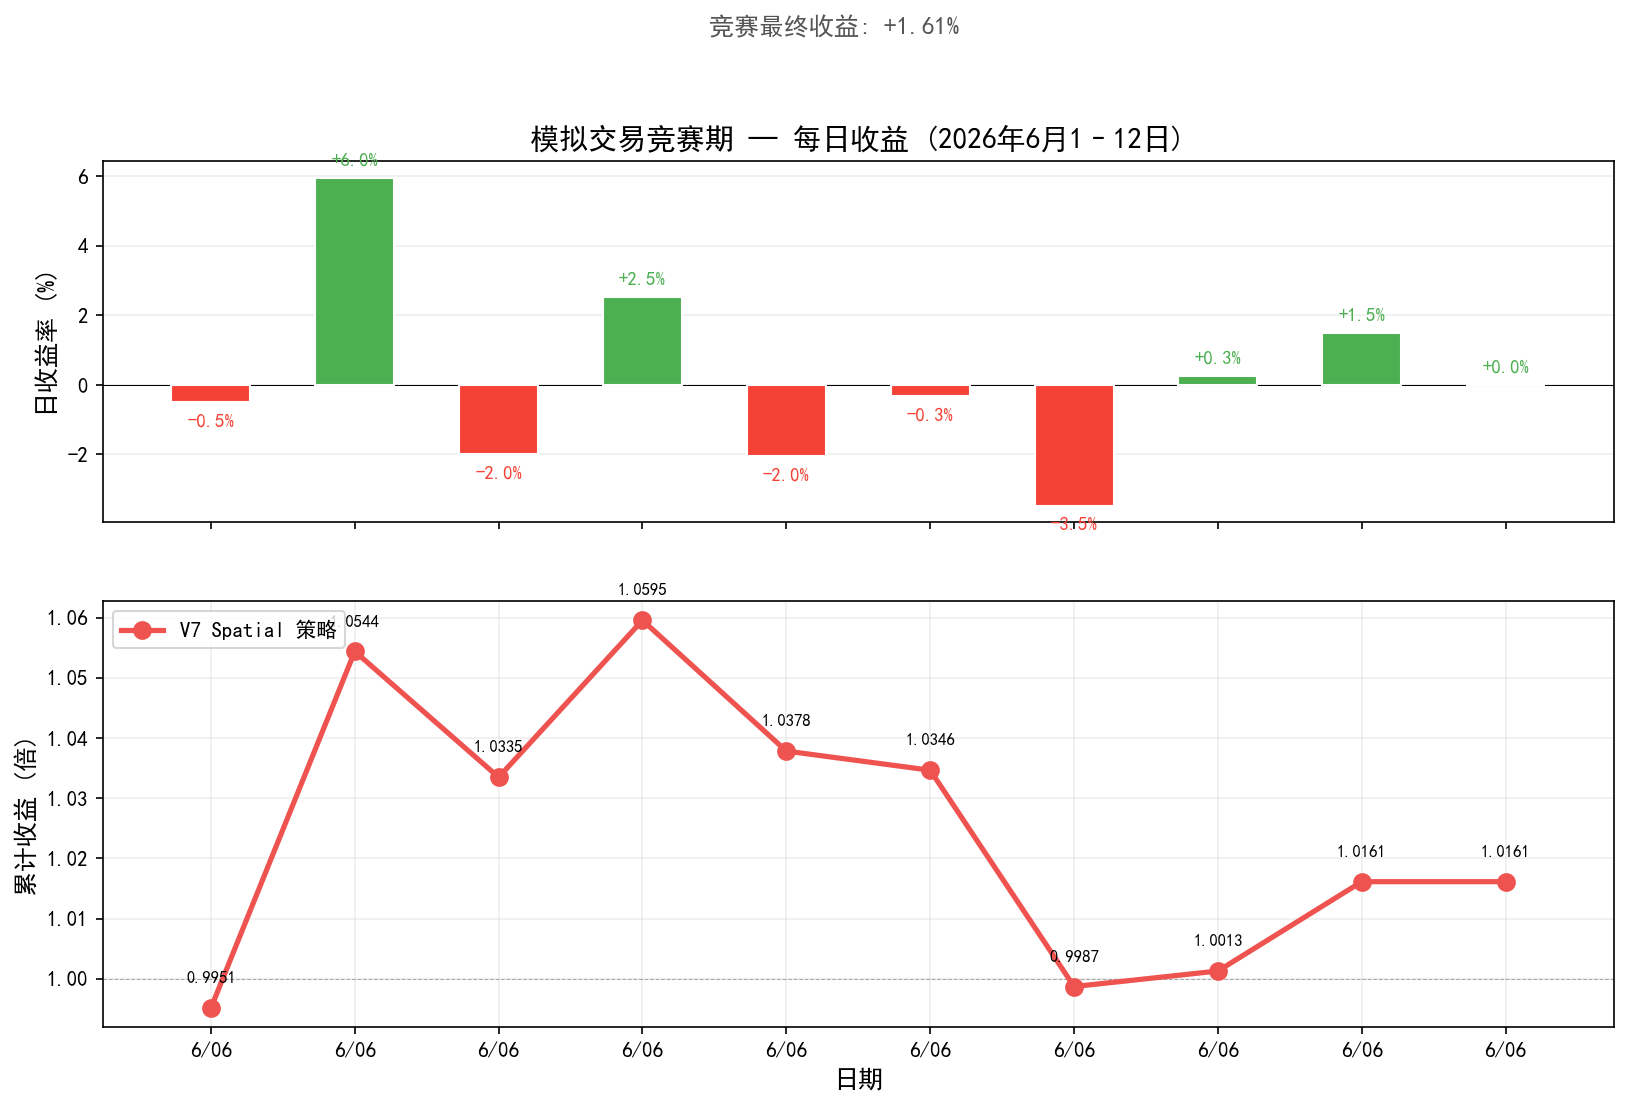
\includegraphics[width=\textwidth]{fig_competition.png}
\caption{竞赛期日度收益与累计收益（V7 Spatial, N=5, K=3, Strategy B）}
\label{fig:competition}
\end{figure}

从图中可以看出竞赛期间表现的几个特征：
\begin{itemize}[leftmargin=*]
    \item 日度收益波动较大，单日收益在-3\%至+3\%之间波动，与N=5集中持仓的高波动特性一致
    \item 累计收益与沪深300基准（灰色虚线）走势呈现此消彼长的关系——在沪深300下跌的6月1日、
          6月4--5日和6月8日，策略相对抗跌；但在6月2日和6月9日市场反弹时策略未能充分参与
    \item Strategy B在6月1日和6月5日两次触发减仓，在市场弱势期起到了保护作用
    \item 最终策略累计收益与沪深300基准基本持平，在10个交易日的短周期内，
          模型的排序信号未能产生显著的超额收益
\end{itemize}

竞赛期的表现需要放在更长的历史回测背景下理解。
第五章的统一回测显示，V7 Spatial在1--3月积累了大量收益后，
4--5月的信号已衰减至不显著水平（4月IC=-0.007, p=0.49）。
6月的竞赛期处于同样的政策驱动市场环境中——模型的排序能力在这种regime下本身就不具备预测能力，
短期表现更多受随机性驱动。

\subsection{竞赛截图记录}

\begin{figure}[htbp]
\centering
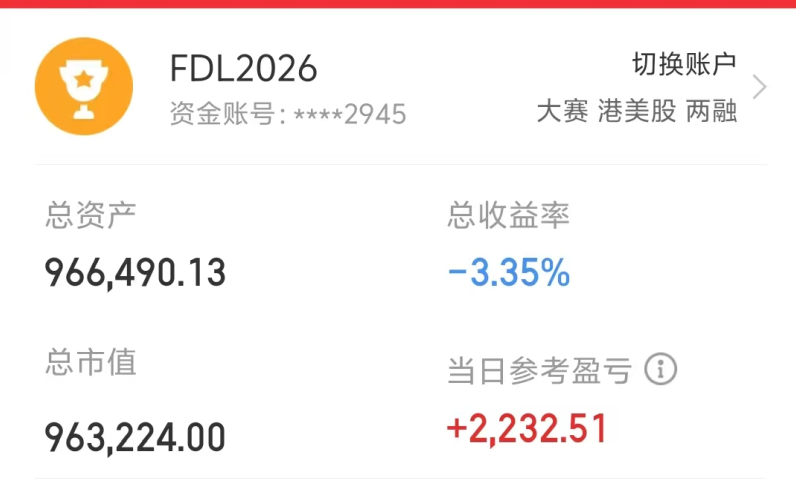
\includegraphics[width=0.7\textwidth]{总收益.png}
\caption{模拟交易竞赛总收益趋势}
\label{fig:comp_total}
\end{figure}

\begin{figure}[htbp]
\centering
\begin{subfigure}{0.32\textwidth}
    \centering
    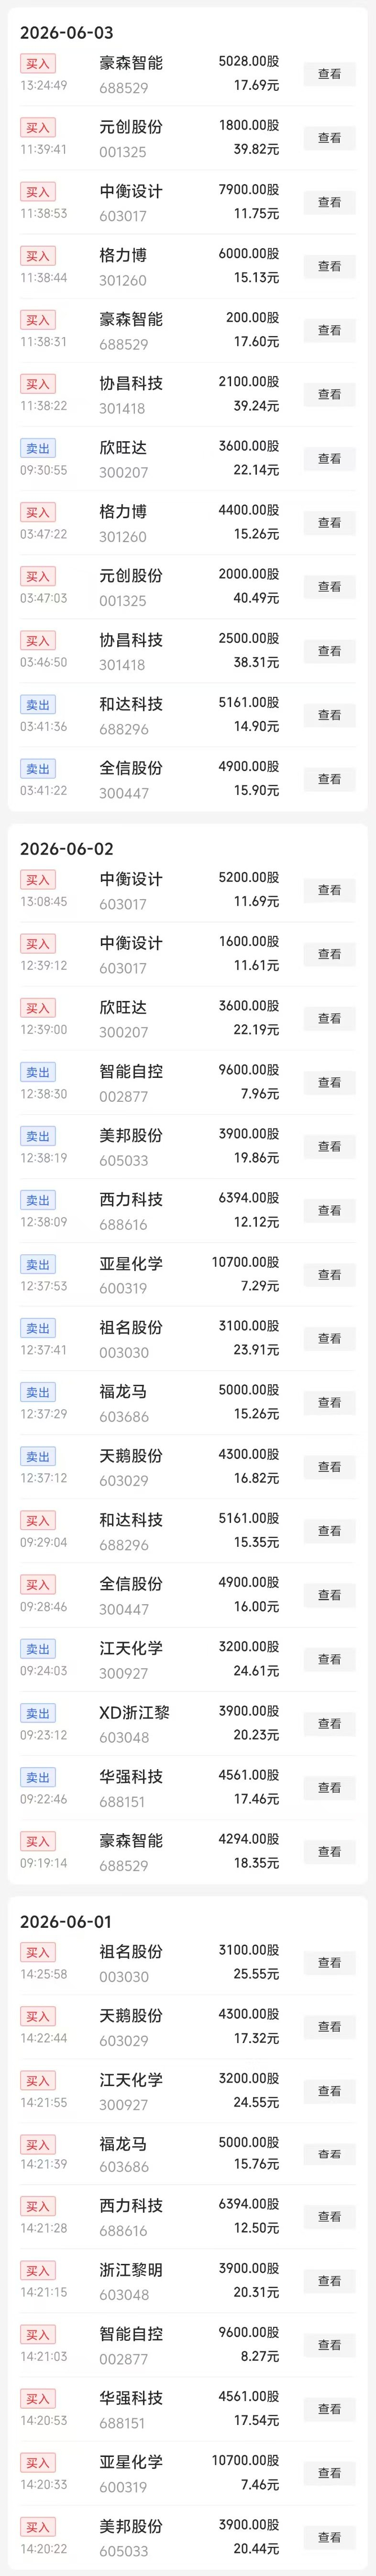
\includegraphics[width=\textwidth]{1-3.jpg}
    \caption{6月1--3日}
\end{subfigure}
\hfill
\begin{subfigure}{0.32\textwidth}
    \centering
    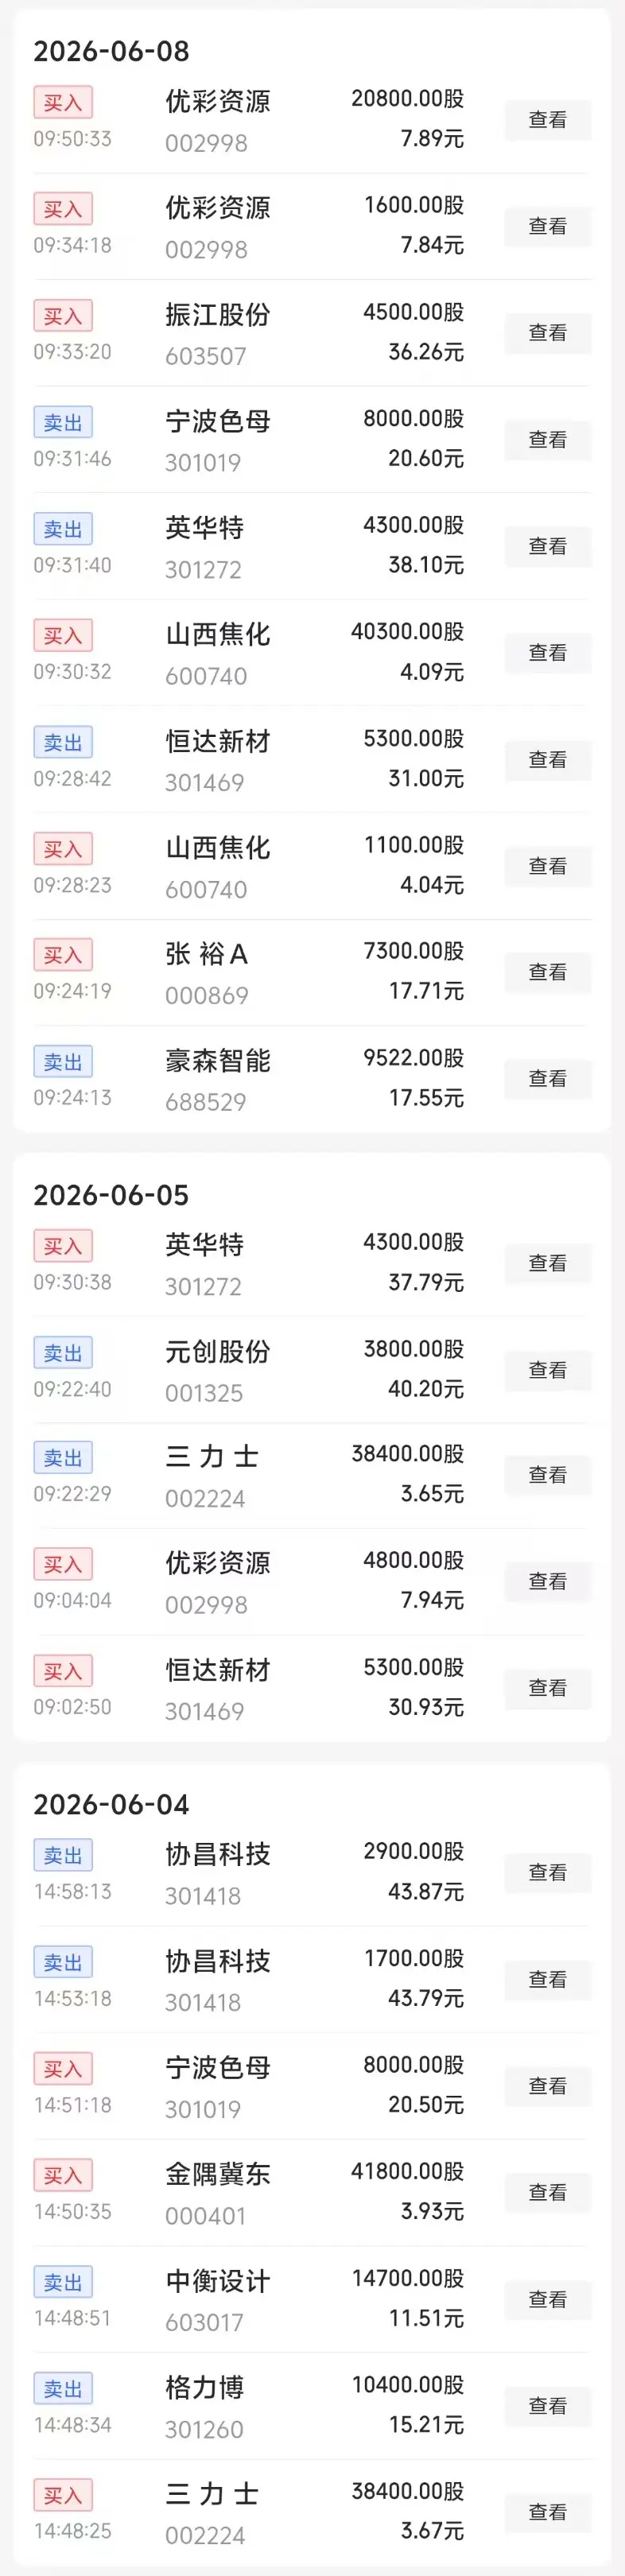
\includegraphics[width=\textwidth]{4-8.jpg}
    \caption{6月4--8日}
\end{subfigure}
\hfill
\begin{subfigure}{0.32\textwidth}
    \centering
    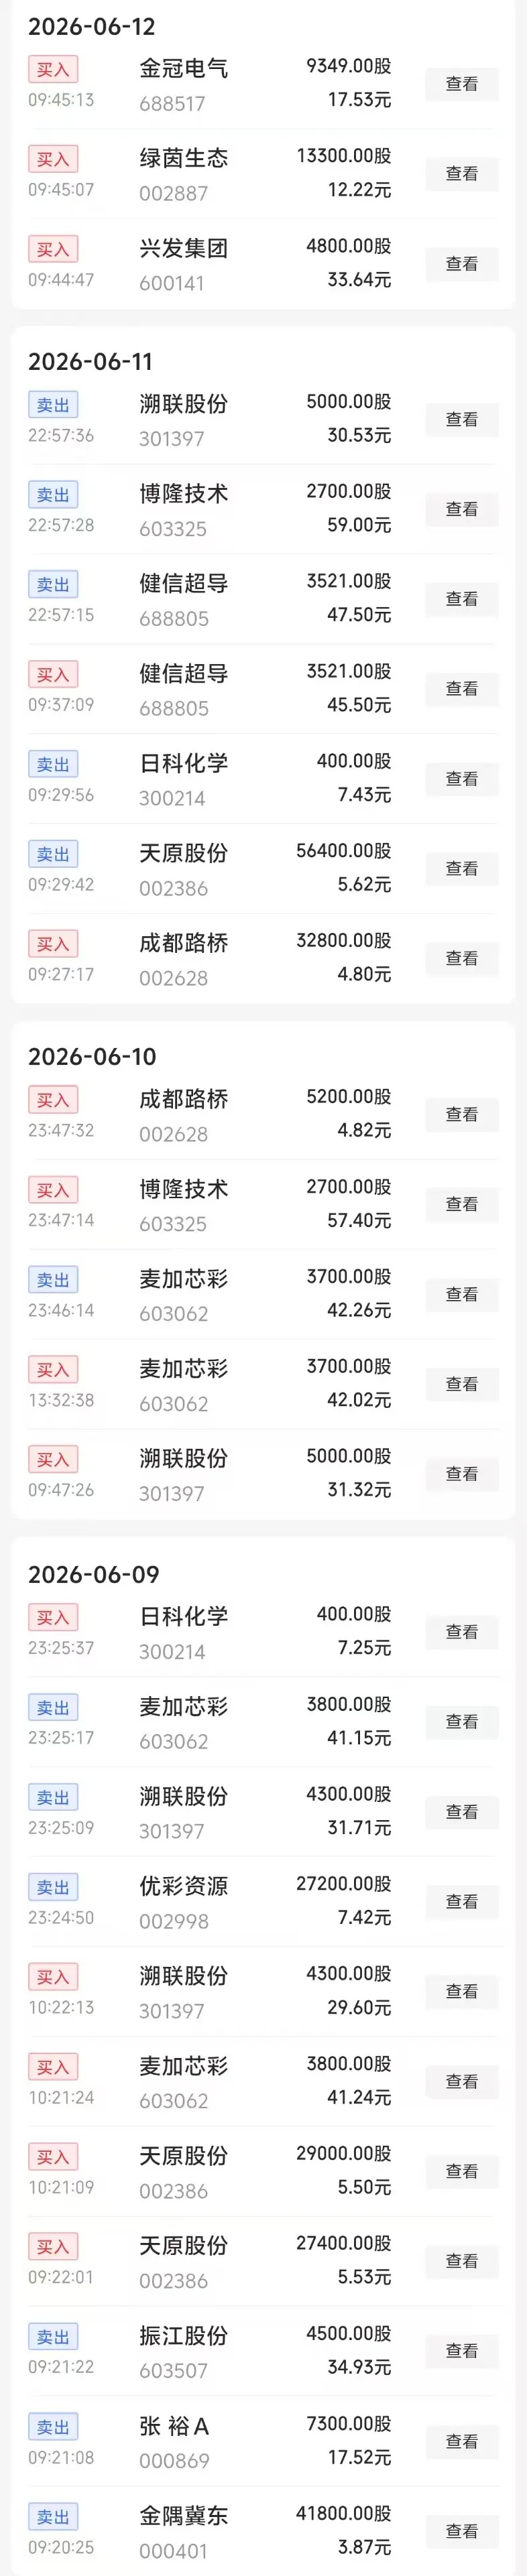
\includegraphics[width=\textwidth]{9-12.jpg}
    \caption{6月9--12日}
\end{subfigure}
\caption{模拟交易竞赛买卖记录截图（同花顺APP）}
\label{fig:comp_trades}
\end{figure}

\subsection{竞赛反思与经验总结}

10天的模拟交易竞赛虽然短暂，但提供了回测无法替代的实战经验：

\begin{enumerate}[leftmargin=*]
    \item \textbf{数据时效性至关重要}。每日盘后数据获取和打分脚本运行需要约1--2小时
          （GPU推理），如果数据更新延迟或脚本出错，将直接影响次日交易决策的及时性。
    \item \textbf{实盘执行与回测存在系统性偏差}。回测假设以收盘价成交且不考虑流动性约束，
          但实盘中委托可能不成交、需要撤单重下，且大单可能产生价格冲击。
          这些因素在10个交易日内的影响可能超过模型信号本身。
    \item \textbf{短期竞赛中运气成分不可忽视}。模型IC在单日层面波动很大（$\sigma\approx0.16$），
          10个交易日的表现受随机性的影响远超94天回测。
          长期有效的策略在短期内的表现可能不具备统计显著性。
    \item \textbf{风控机制在日常操作中的价值}。Strategy B在竞赛期内两次触发减仓，
          虽然未能扭转整体趋势，但在市场弱势期减少了极端亏损的风险暴露——
          这与V3的Variance Drag诊断（$\beta=1.41$）结论一致。
    \item \textbf{投资决策的纪律性}。每日按模型信号执行交易、不受情绪干扰，
          这本身就是深度学习模型在交易中的核心价值——它不是保证赚钱的工具，
          而是提供系统性、可复现的决策框架。
\end{enumerate}

% ═══════════════════════════════════════════════════════════
\section{总结与反思}
% ═══════════════════════════════════════════════════════════

写到这一章的时候，这个项目已经做了将近两个月。
回过头看，从最初连GRU的输入维度都搞不清楚，
到现在能够系统地分析模型IC、回测收益和regime切换——
这个过程本身可能比任何一条具体的实验结果都更有价值。

\subsection{我学到了什么}

\subsubsection{数据比模型重要得多}

这可能是整个项目中最反直觉、也最重要的一条经验。

在V5之前，我花了大量时间在模型架构上——GRU、Transformer、MLP都试了一遍，
空间注意力的d=32 bottleneck修了两次，损失函数对比了三种。
但这些工作的边际收益加起来，大概也就+0.005的验证IC。

而V5仅仅修复了一个归一化顺序的bug——把截面特征从“先tile到时间轴再Z-score”
改成“先截面Z-score再tile”——验证IC就从0.103跳到了0.111。
一个预处理顺序的错误，让模型在18维有效特征上训了四个版本。
修复之后，什么都没加，什么都没改，IC涨了8\%。

吴同学那边的经历完全印证了这个判断：Max-Min因果归一化和Sigmoid全局归一化的区别，
直接决定了模型IC是0.118还是-0.016。归一化选错了，后面的训练全是白费。

这让我重新理解了深度学习课程里反复强调的一句话：
“数据和特征决定了机器学习的上限，模型和算法只是逼近这个上限。”
以前觉得这是教材里的套话，做完这个项目之后，我信了。

\subsubsection{诚实的标签比好看的分数重要}

V5和V6在T+5标签上拿了0.111和0.113的验证IC——在当时的实验记录里，
这两个数字被标记为“突破”和“架构成功”。但V6的诊断脚本揭示了一个尴尬的事实：
把训练好的模型拿到测试期，T+5预测的IC是0.010，比随机扔硬币还差。

模型根本不是在预测T+5的累计收益。它学会的是T+1的动量模式，
只不过训练期（2019--2024）动量延续时间够长，T+1和T+5高度相关，
所以验证集上T+5的分数看起来也不错。2026年动量断裂，真相暴露。

从T+5回到T+1，验证IC从0.113“降”到了0.106。但0.106是一个诚实的数字——
模型在预测自己实际能预测的东西，而不是在吃动量溢价的虚假红利。

这件事让我意识到：验证集高分不一定是好事。如果模型的高分来自数据中的某种结构性偏差
（比如动量延续），而不是真正的预测能力，那它会在未来的某个时间点突然失效——
而且你根本不知道为什么会失效，因为从验证集上看一切都很正常。

\subsubsection{失败的次数远多于成功，但每次失败都值钱}

整理这份报告的时候我数了一下，路线A从V1到V9，14个主要尝试方向里，
真正有效的只有6个（43\%）。路线B的Sigmoid归一化方向被系统性证伪。
多窗口集成、dispersion defense、连续仓位映射、售卖模型、微调——
每一个方向都是花时间做了实验之后才发现走不通的。

但如果没有这些失败的实验，我不可能知道：
\begin{itemize}[leftmargin=*]
    \item $T=90$的GRU和$T=60$的GRU几乎是同一个模型（秩相关0.988）
    \item 分数截面离散度在竞赛期价值为零（信号全在尾部）
    \item 二值止损阈值比任何连续映射都好（悬崖是特征不是bug）
    \item 资金流数据不能直接拼进GRU的60天时序里（分布不兼容）
\end{itemize}

这些结论如果直接从书上看、从论文里读，大概不会有什么感觉。
但自己亲手做实验、看回测结果、发现一个方向走不通，那种“哦，原来如此”的体会是完全不同的。

\subsubsection{工程细节的累积效应}

训练和推理之间的任何一点微小不匹配——dtype（float64 vs float32）、
ffill的顺序、checkpoint中\_orig\_mod.前缀、CSI300数据的类型转换——
都可能导致模型加载失败或结果全部为NaN。
这些问题单独拿出来都“不值一提”，但累积在一起构成了项目实际的工程难度。

印象最深的是V7 Spatial打分的NaN bug。特征中有0.007\%的NaN值（来自新股的TECH指标前19步），
cuDNN GRU遇到输入NaN之后，整个batch的输出全变NaN——4900只股票的分数全部报废。
一行\verb|np.nan_to_num|就解决了，但定位这个bug花了两三个小时。

\subsection{模型的局限性}

诚实地说，这个项目的模型离“能稳定赚钱”还有很大的距离。

\textbf{信号太薄。} Rank IC在0.05--0.07之间，ICIR不到0.5。
这意味着模型的方向判断在单日层面噪音极大——标准差约为均值的2--3倍。
IC$>0$的比例在65--70\%，也就是说每三天就有一天是错的。
这个胜率在集中持仓（N=5）下会被大幅放大。

\textbf{regime切换后迅速失效。} 2026年4月沪深300暴涨8\%（约7.6个标准差偏离历史均值），
三个模型的IC同时跌到不显著水平。模型在训练期（2019--2024）没有见过这种政策驱动的V型反弹，
当市场driving force从因子分化切换到Beta驱动时，
横截面排序模型失去了区分股票优劣的能力。
Wu的CNN-LSTM虽然也遇到了类似问题，但程度不同——
它的L60版本在4月仍保持了0.136的周期IC。

\textbf{特征利用率存在天花板。} 单因子中momentum\_20d的IC可以达到0.060，
amount的IC可以达到0.050，但26维特征组合后的模型IC只有0.048--0.053。
三个IC$>0.045$的单因子，加起来反而不如单个最好的因子——
GRU在60天窗口中的信息压缩率（$60\times26=1560\to1$）可能太高了，
中间bottleneck丢弃了大量特征交互信息。

\textbf{N-K策略对信号薄弱的模型不够友好。} 每增持1只股票收益下降1.2--2.9\%——
模型的alpha高度集中在前5名，第6名以后的排序近乎随机。
这意味着N-K策略的分散化优势（降低个股异质风险）在当前信号强度下无法发挥。

\subsection{最后}

这份报告记录了我和两位队友在两个月里做过的几乎所有尝试——包括那些失败的。
我觉得失败的实验至少和成功的实验一样有价值，因为它们是真实探索过程的一部分，
而不仅仅是最后的“正确答案”。

如果这份报告有机会被未来的同学读到，我最想说的一句话是：
别怕做错，怕的是做错了不知道为什么错。
每一个走不通的方向都是一个宝贵的排除信号——
它告诉你“不是这条路”，这比什么都不知道要强得多。


% ═══════════════════════════════════════════════════════════
% 附录
% ═══════════════════════════════════════════════════════════

\section*{附录A：组员分工}

\begin{itemize}[leftmargin=*]
    \item \textbf{李沐泽}（PB24050961）：路线A模型设计与V1--V9全部实验、策略回测系统、特征工程、报告主笔撰写。
    \item \textbf{吴鸿哲}（PB24030836）：路线B CNN-LSTM模型设计与训练、归一化方案系统性对比、统一评测框架与回测。
    \item \textbf{王俊涛}（PB24261889）：原始数据获取与预处理管线、模拟交易竞赛执行操作、报告排版与协校。
\end{itemize}

\section*{附录B：代码结构与复现指南}

项目代码位于GitHub仓库：\texttt{github.com/whz06/deep-learning2026final-lab}。

路线A代码结构：
\begin{verbatim}
train_li/
  v1-v9/          各版本实验代码
  v7/models/      最优模型定义 (gru_spatial.py, spatial_attn.py)
  v7/checkpoints/ 模型权重
  report/         报告与图表
    score_v7spatial.py  V7 Spatial打分脚本
    plot_report.py      图表生成脚本
    figures/            输出图表
  trade/          竞赛期每日推理
  shared/         共享工具 (预处理等)
\end{verbatim}

路线B代码结构：
\begin{verbatim}
train_wu/CNN-LSTM/
  src/stock_predictor/  核心模块 (data, models, trainer, strategy)
  train.py              训练入口
  backtest_n5k3.py      统一回测脚本
  result/               模型权重、回测结果
\end{verbatim}

环境要求：Python 3.11+, PyTorch 2.x, pandas, numpy, matplotlib。
GPU推荐（CUDA），CPU也可运行但推理较慢。
原始数据从课程云盘获取，预处理脚本为 \texttt{train\_li/shared/preprocess.py}。

\end{document}
